\documentclass[letterpaper, 11pt]{article} 

\usepackage{graphics,graphicx}
\usepackage{multicol} 
\usepackage{parskip}
\usepackage{amsmath}
\usepackage{multirow}
\usepackage[utf8]{inputenc}
\usepackage{fancyhdr}
\usepackage[title]{appendix}
\usepackage{wasysym}
\usepackage{url}
\usepackage{subcaption}

\usepackage[font=footnotesize,labelfont=small]{caption}
\usepackage{longtable}
\captionsetup{width=0.85\linewidth}

\RequirePackage{geometry}
\geometry{margin=2cm}

\setlength{\parskip}{0.2cm}
\setlength{\parindent}{0pt}

\newcommand{\HRule}[1]{\rule{\linewidth}{#1}}
\newcommand{\subsubsubsection}[1]{\paragraph{#1}\mbox{}\\}
\setcounter{secnumdepth}{4}

\begin{document}
	
	\title{ 
		\normalsize \textsc{ECEC 572 - Custom VLSI Design \& Analysis}
		\\ [2.0cm]
		\HRule{0.5pt} \\
		\LARGE \textbf{\uppercase{Final Report}} \\
		\normalsize  \vspace*{1\baselineskip}
		\LARGE \textbf{\uppercase{VLSI Design of a Visible Watermarking Processor}}
		\HRule{2pt} \\ [0.5cm]
		\normalsize  \vspace*{5\baselineskip}
		\textsc{Drexel University, College of Engineering} \\
		\normalsize  \vspace*{7\baselineskip}
	}
	
	\author{
		Group 2: \\
		Hieu Mai (hqm23)\\
		Tai Nguyen (tdn47)  \\
		Quang-Anh Hoang (qh62) \\
		Hanh Do-Phung (hdd29)\\ 
	}
	
	\date{March 18, 2021}
	
	\maketitle
	\newpage
	
	\tableofcontents
	\newpage
	
	\rule{\textwidth}{1pt}
	
	\section{Background}
	\label{sec:background}
	
	%\begin{multicols}{2}
	Watermarking is the process of embedding data (visible or hidden) into a different piece of information in order to verify or control such information’s distribution. This operation is most commonly done on photos or videos in order to protect their copyright. A hidden watermark is imperceptible to the human eye but a visible one is often translucent and overlaid onto the original medium. In this project, we followed a paper by Mohanty and Namballa \cite{1} designed, implemented, and tested a processor which applies a visible watermark onto an input image in real-time.
	
	The author of \cite{1} mentioned 2 different methods, one simple, one more complex to perform watermarking. The simple method only involves adding a gray-scaled value of the watermark pixel into the host pixel in a way that the final image is still perceptually comparable to its original version. A simple algorithm is introduced by Meng and Chang \cite{2} and is summarized by the equation below:
	
	\begin{equation}
		I_{W(m,n)}=\begin{cases}
			I(m,n) + W(m,n)(\frac{I_{white}}{38.667})(\frac{I(m,n)}{I_{white}}), & \text{for } \frac{I(m,n)}{I_{white}} > 0.008856\\
			I(m,n) + W(m,n)(\frac{I(m,n)}{903.3})\alpha_I, & \text{for } \frac{I(m,n)}{I_{white}} \leq 0.008856
		\end{cases}
	\end{equation}
	
	Where $I_w$ is the final watermarked image, $I$ is the original image, $W$ is the watermark image, and $\alpha_I$ is a global scaling factor. Assuming $I_{white}=255$, It can be simplified further into
	
	\begin{equation}
		I_{W(m,n)}=\begin{cases}
			I(m,n) + (\frac{\alpha_I}{6.0976})W(m,n)I(m,n)^{2/3}, & \text{for } I(m,n) > 2.2583\\
			I(m,n) + (\frac{\alpha_I}{903.3})W(m,n)I(m,n), & \text{for } I(m,n) \leq 2.2583
		\end{cases}
	\end{equation}
	
	However, as cube root is involved, it could be difficult to implement in hardware. Hence, the author divided the piece-wise equation into 4 parts instead of 2 to reduce complexity:
	
	\begin{equation}
		\label{eq3}
		I_{W(m,n)}=\begin{cases}
			I(m,n) + (\frac{\alpha_I}{903.3})W(m,n)I(m,n), & \text{for } I(m,n) \leq 2 \\
			I(m,n) + (\frac{\alpha_I C_1}{6.0976})W(m,n)I(m,n), & \text{for } 2 < I(m,n) \leq 64 \\
			I(m,n) + (\frac{\alpha_I C_2}{6.0976})W(m,n)I(m,n), & \text{for } 64 < I(m,n) \leq 128 \\
			I(m,n) + (\frac{\alpha_I C_3}{6.0976})W(m,n)I(m,n), & \text{for } 128 < I(m,n) \leq 192 \\
			I(m,n) + (\frac{\alpha_I C_4}{6.0976})W(m,n)I(m,n), & \text{for } 192 < I(m,n) \leq 256 \\
		\end{cases}
	\end{equation}
	
	$C_1, C_2, C_3, C_4$ are linear regression coefficients that best approximate the cube root. The authors in \cite{1} found through simulations that 0.339644, 0.21988, 0.185746, and 0.172925 are good values for $C_1, C_2, C_3, C_4$, respectively.
	
	The second algorithm is proposed in [3] by Mohanty et.al and it involves the following steps:
	
	\begin{enumerate}
		\item Both the original image and the watermark image is divided into blocks of equal sizes
		\item The local statistics: mean, variance are computed for each block of each image.
		\item If $I_{Wk}$ is the kth block of the final image, then: $I_{Wk}=\alpha_k I_k + \beta_k W_k$, where $\alpha_k$ and $\beta_k$ depends on the calculated local statistics.
	\end{enumerate}
	
	Since the choice of $\alpha_k$ and $\beta_k$ is governed by the human vision system (HVS), the authors in \cite{3} proposed that: $\alpha_k=\alpha_{max}$ and $\beta_k=\beta_{min}$ if the block k is an \textbf{edge} block. Otherwise, they are calculated such that: 
	
	\begin{equation}
		\begin{aligned}
			& \alpha_k = \frac{1}{\hat{\sigma_{kI}}} exp(-(\hat{\mu_{kI}} - \hat{\mu{I}})^2) \\
			& \beta_k = \hat{\sigma_{kI}} (1 - exp(-(\hat{\mu_{kI}} - \hat{\mu{I}})^2))
		\end{aligned}
	\end{equation}
	
	Then, they are scaled to their max and min range:
	
	\begin{equation}
		\begin{aligned}
			& \alpha_k = (\frac{\alpha_{max} - \alpha_{min}}{\alpha^c_{max} - \alpha^c_{min}})\alpha^c_k + (\alpha_{max} - (\frac{\alpha_{max} - \alpha_{min}}{\alpha^c_{max} - \alpha^c_{min}})\alpha^c_{max}) \\
			& \beta_k = (\frac{\beta_{max} - \beta_{min}}{\beta^c_{max} - \beta^c_{min}})\beta^c_k + (\beta_{max} - (\frac{\beta_{max} - \beta_{min}}{\beta^c_{max} - \beta^c_{min}})\beta^c_{max})
		\end{aligned}
	\end{equation}
	
	Where $\alpha_k^c$ and $\beta_k^c$ are current values before scaling, $\alpha_{max}^c$, $\alpha_{min}^c$, $\beta_{max}^c$, and $\beta_{min}^c$ are current known max and min values of $\alpha$ and $\beta$. However, in order to calculate these values, the algorithm needs to go through all the blocks first. This can be slow and inefficient. Hence, the authors in \cite{1} provided an approximation in which they claimed would be within 5\% of the original algorithm:
	
	\begin{equation}
		\label{eq6}
		\begin{aligned}
			& \alpha_k = \alpha_{min} + (\alpha_{max} - \alpha_{min})\frac{1}{\hat{\sigma_{kI}}} exp(-(\hat{\mu_{kI}} - \hat{\mu{I}})^2) \\
			& \beta_k = \beta_{min} + (\beta_{max} - \beta_{min})\hat{\sigma_{kI}} (1 - exp(-(\hat{\mu_{kI}} - \hat{\mu{I}})^2))
		\end{aligned}
	\end{equation}
	
	The exponential function is also approximated using Taylor series in order to make the hardware implementation simpler and faster:
	
	\begin{equation}
		\label{eq7}
		e^x = \sum_{i}\frac{x^i}{i!} = 1 + x + \frac{1}{2}x^2 + ...
	\end{equation}
	
	With these 2 algorithms, Mohanty and Namballa \cite{1} proposed a VLSI chip design which lets the user choose between them.
	
	\section{Specification}
	\label{sec:specs}
	
	According to the 2 algorithms above, the overall high-level circuit is summarized in the figure \ref{fig1} below:
	
	\begin{figure}[htb!]
		\centering
		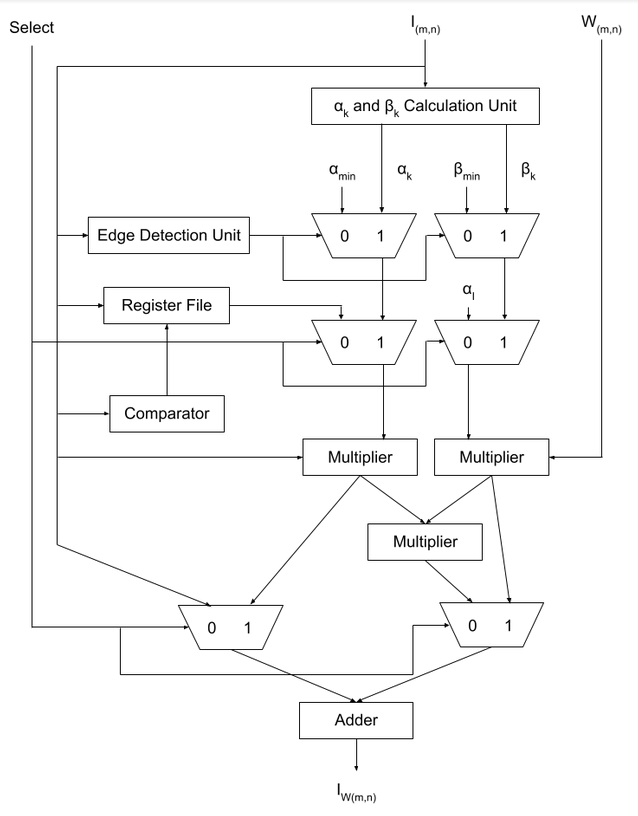
\includegraphics[width=0.4\linewidth]{report_pics/overall_block_diagram.png}
		\caption{Overall datapath block diagram (reproduced from paper \cite{1})}
		\label{fig1}
	\end{figure}
	
	There are 3 main blocks:
	
	\begin{enumerate}
		\item $\alpha_k$ and $\beta_k$ calculation unit
		\item Edge detection unit
		\item Register file
	\end{enumerate}
	
	The block diagram for the $\alpha_k$ and $\beta_k$ calculation unit (figure \ref{fig2a}) and the edge detection unit (figure \ref{fig2b}) is:
	
	\begin{figure}[ht!]
		\centering
		\begin{subfigure}[b]{.35\linewidth}
			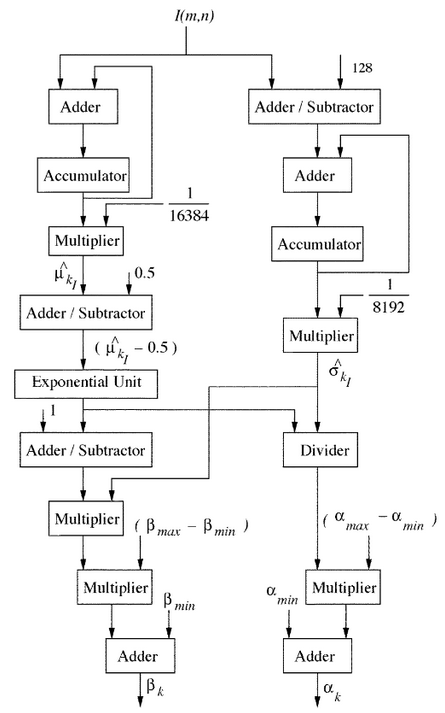
\includegraphics[width=\textwidth]{report_pics/ak_bk_unit_block_diagram.png}
			\caption{}
			\label{fig2a}
		\end{subfigure}
		%	\hskip2em
		\begin{subfigure}[b]{.35\linewidth}
			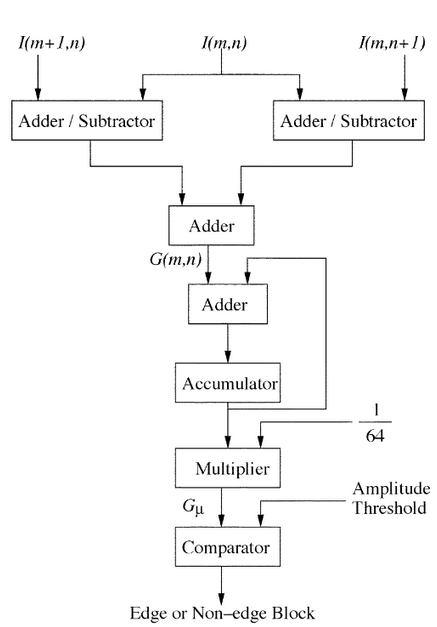
\includegraphics[width=\textwidth]{report_pics/edge_unit_block_diagram.png}
			\caption{}
			\label{fig2b}
		\end{subfigure}
		\caption{(a) $\alpha_k$ and $\beta_k$ calculation unit and (b) edge detection unit's block diagram (from paper \cite{1})}
	\end{figure}
	
	We first explored SRAM as our register file design. However, due to the complexity of SRAM as a semi-analog device and the amount of work which had to be done on the controller's side (we aim for the controller to only be a finite state-machine without any memory timing controls), we decided to stick with the simplistic DFF design as a memory cell. However, since we need to be able to write into a cell and read from it at any time (however, not at the same time), we realized that we need to include tri-state buffers in order to control the flow of the data in and out of the DFF. Through research we found a design principle from a math course at Emory University \cite{4} that suits our need (figure \ref{fig3}): 
	\newpage
	\begin{figure}[htb!]
		\centering
		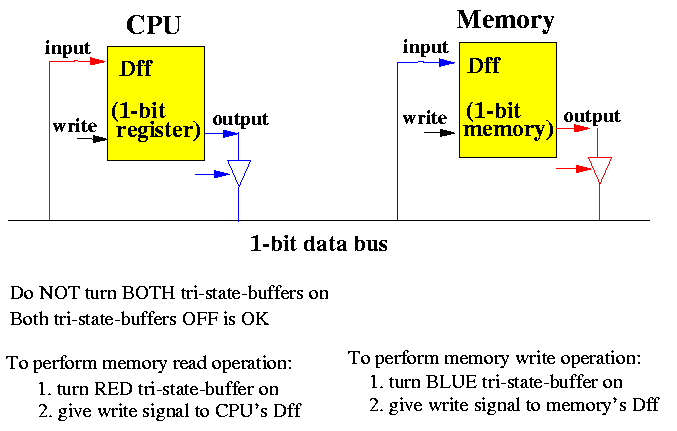
\includegraphics[width=0.5\linewidth]{report_pics/tristate_emory.png}
		\caption{A memory design principle from a math course at Emory University \cite{4}}
		\label{fig3}
	\end{figure}
	
	In essence, the tri-state buffers (tri-buf) act similar to a variable resistor in which if enabled then they allow inputs to flow through and otherwise, if disabled, then they work as if the wire is disconnected. Hence, if we have 2 tri-state buffers, one controlled by CPU and the other one controlled by the memory cell, then we can read and write to the DFF by controlling these 2 wires.
	
	However, since we do not want to allow the cell to keep outputting while (or immediately after) it is being written to, we included one more tri-buf at the end which is controlled by a read\_enable signal (Figure \ref{fig4a})
	
	\begin{figure}[ht!]
		\centering
		\begin{subfigure}[b]{.4\linewidth}
			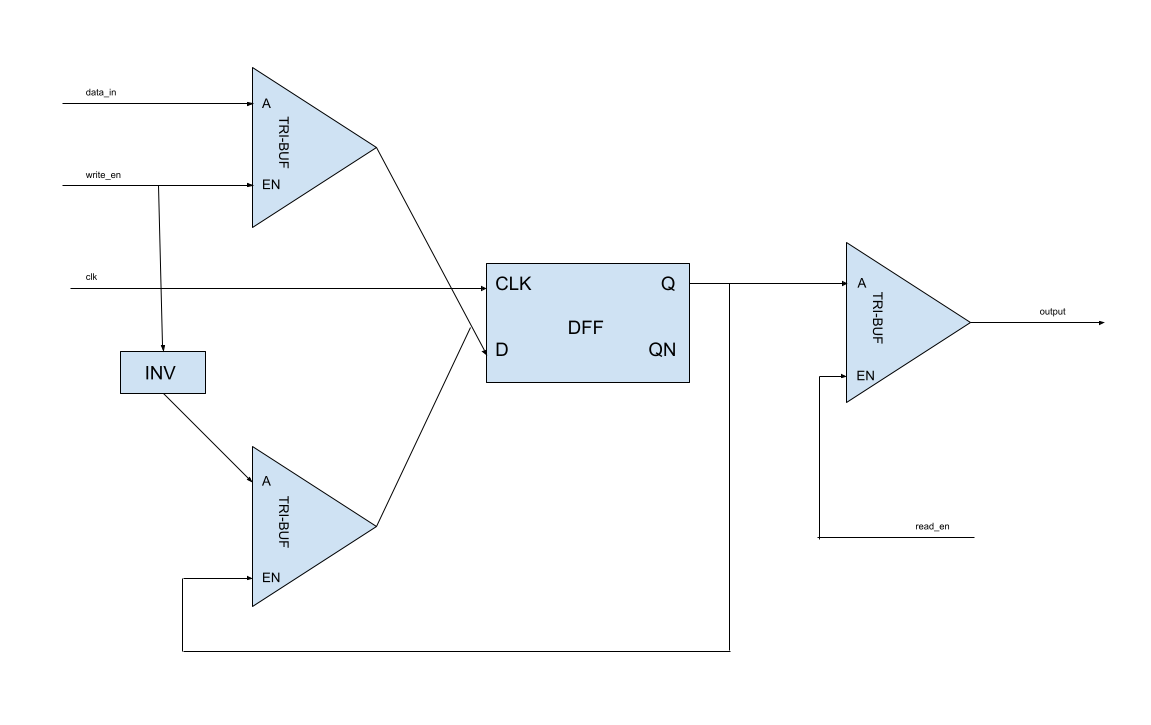
\includegraphics[width=\textwidth]{report_pics/memcell_block_diagram.png}
			\caption{}
			\label{fig4a}
		\end{subfigure}
		%	\hskip2em
		\begin{subfigure}[b]{.4\linewidth}
			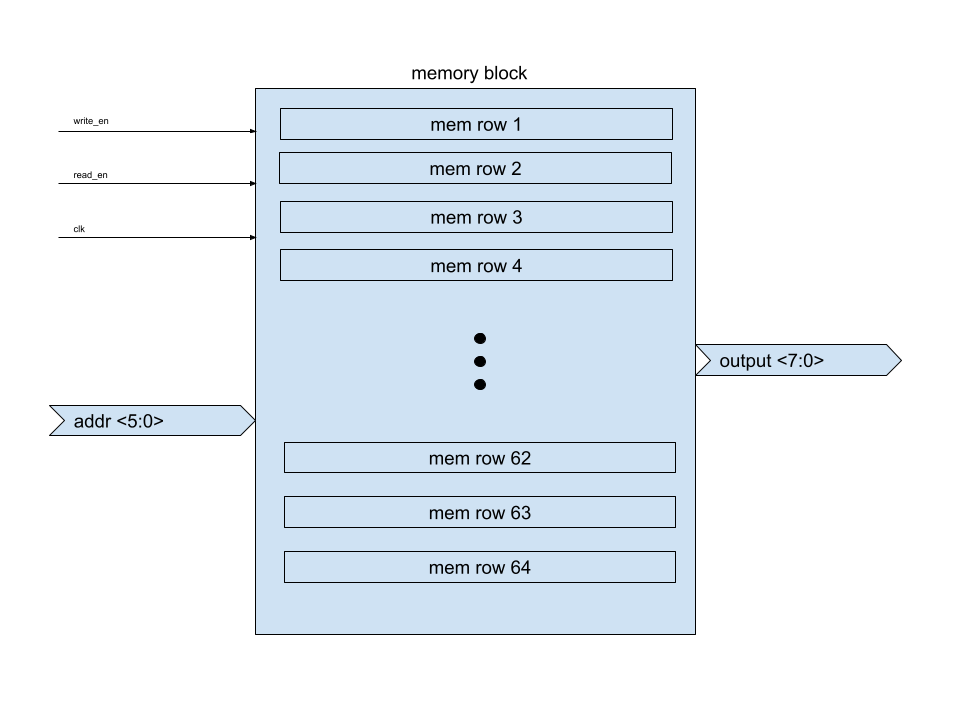
\includegraphics[width=\textwidth]{report_pics/memblock_block_diagram.png}
			\caption{}
			\label{fig4b}
		\end{subfigure}
		\caption{(a) Our memory cell design and (b) a memory block}
	\end{figure}
	
	Using this design, we built a memory row consisted of 8 memory cells, which is going to represent 8 bits, or 1 byte. After that, we created a memory block with 64 memory rows and have a 6-to-64 decoder in order to make our block byte-addressable (Figure \ref{fig4b}).
	
	\section{Design}
	\label{sec:design}
	
	In order to collaborate on this project, we have decided to use the open-sourced Nangate Open Cell Library.
	
	\subsection{Arithmetic Blocks}
	\label{subsec:arith_blocks}
	
	\subsubsection{8-bit Adder-subtractor}
	This arithmetic block is used ubiquitously throughout our designs. Hence, we have carefully considered different adder designs that optimize for speed. We settled upon the design of the carry-look-ahead adder which is the fastest known adder \cite{5}. The design is more complex than the ripple-carry adder but it is better in terms of gate count and delays. Then, we also incorporated subtracting into our adder, making it an adder-subtractor. This design consideration is especially useful and saved a lot of time since it can now be reused in blocks such as: comparator, divider, absolute difference.
	
	In order to add ($A + B$), the control signal should be 0 and otherwise, 1, to subtract ($A - B$). If the subtraction results in a negative number ($A < B$), then the carry out will be 0. If otherwise ($A \geq B$), then the carry out will be 1.
	
	\begin{figure}[htb!]
		\centering
		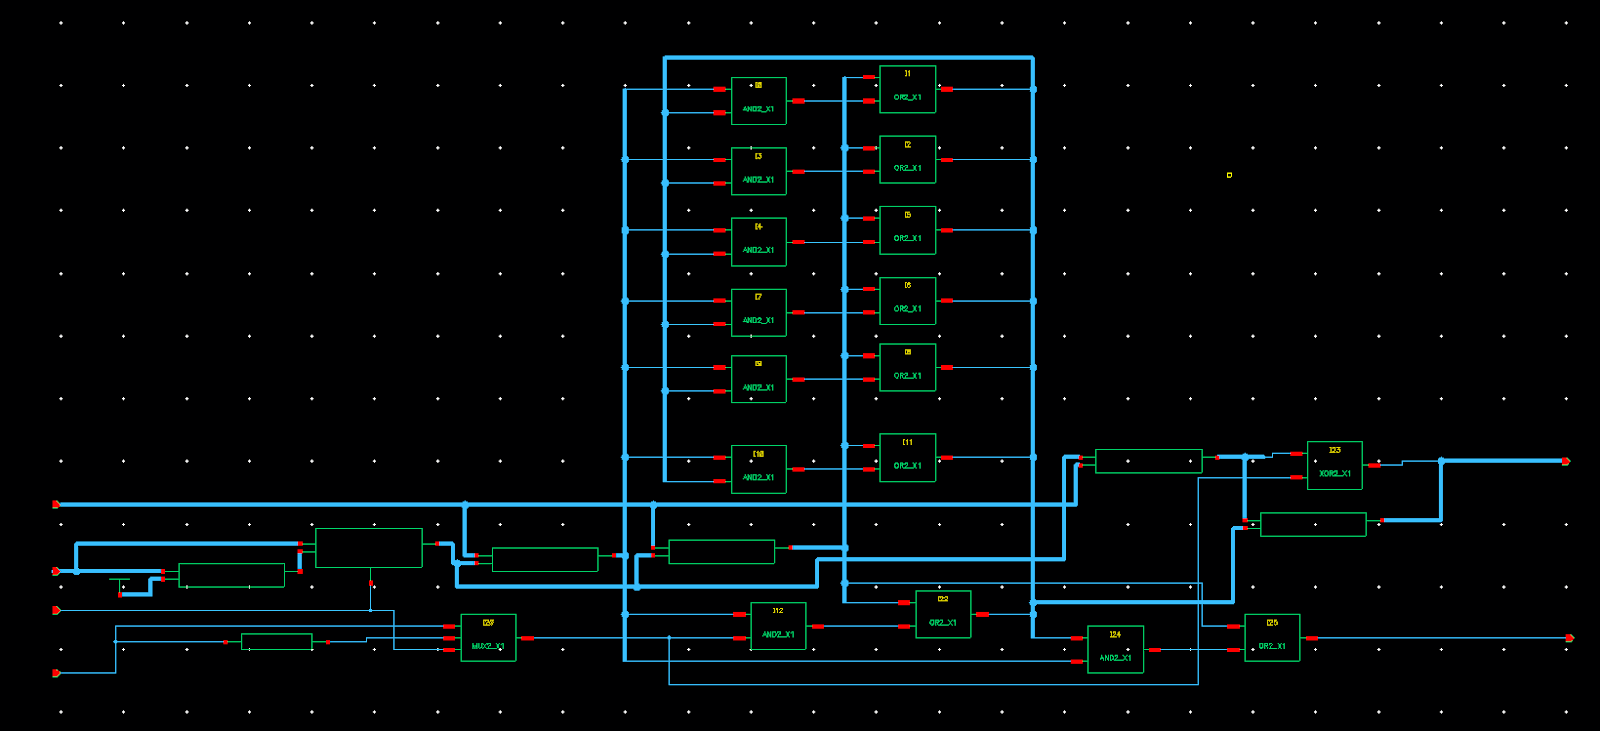
\includegraphics[width=0.85\linewidth]{report_pics/addsub8b_schem.png}
		\caption{8-bit Adder-subtractor schematic design in Cadence}
		\label{fig5}
	\end{figure}
	
	\subsubsection{16-bit Adder}
	The 16-bit adder consists of 2 cascaded 8-bit adder-subtractor(s) with their control signal tied to ground to always enable addition operation. 
	
	\begin{figure}[htb!]
		\centering
		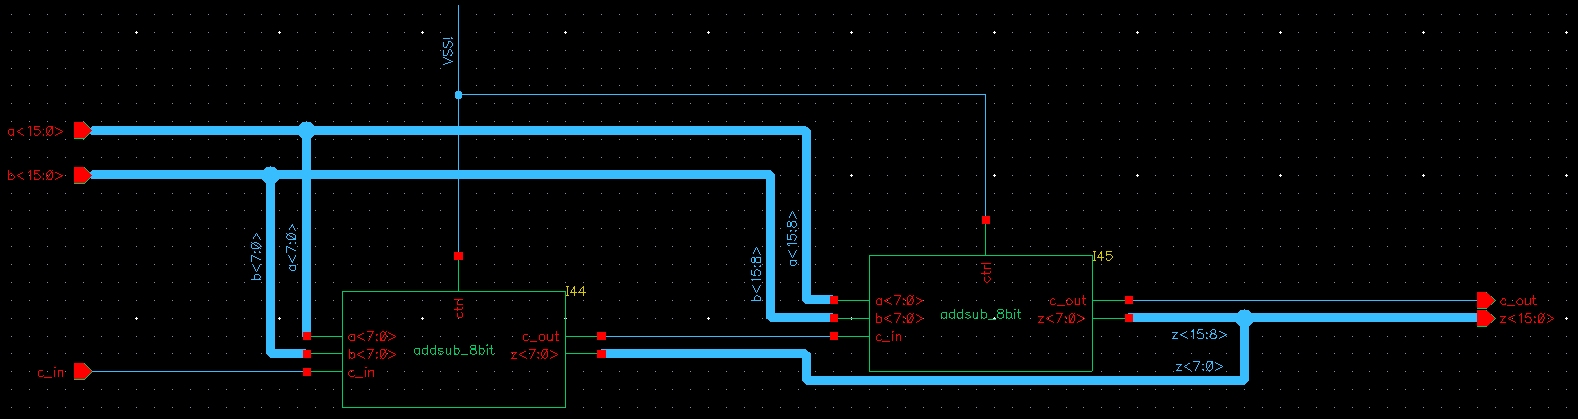
\includegraphics[width=0.85\linewidth]{report_pics/add16b_schem.png}
		\caption{16-bit adder schematic design in Cadence}
		\label{fig6}
	\end{figure}
	
	\newpage
	\subsubsection{16-bit Accumulator}
	The accumulator used in this design is 16-bit due to the need to accumulate 64 8-bit numbers, which would reach a maximum value of 16384 (14 bits). For simplicity, the design choice of 16 bits instead of 14 bits was made as a 16-bit accumulator can easily be based on two 8-bit adders that we can reuse from past designs. 
	
	The 16-bit accumulator uses a 16-bit adder (constructed from the 8-bit add/sub block), and a 16-bit D-Flip flop to store the accumulated number. Also, it has some MUXes in order to allow for the capability to reset, and to freeze the result. If reset is HIGH, then the result will be 0. And if enable is LOW, then the result will stop accumulating per clock cycle (positive edge). This is necessary because algorithm 2 requires the arithmetic to be done in stages and we do not want the result of the next stage to change.
	
	\begin{figure}[htb!]
		\centering
		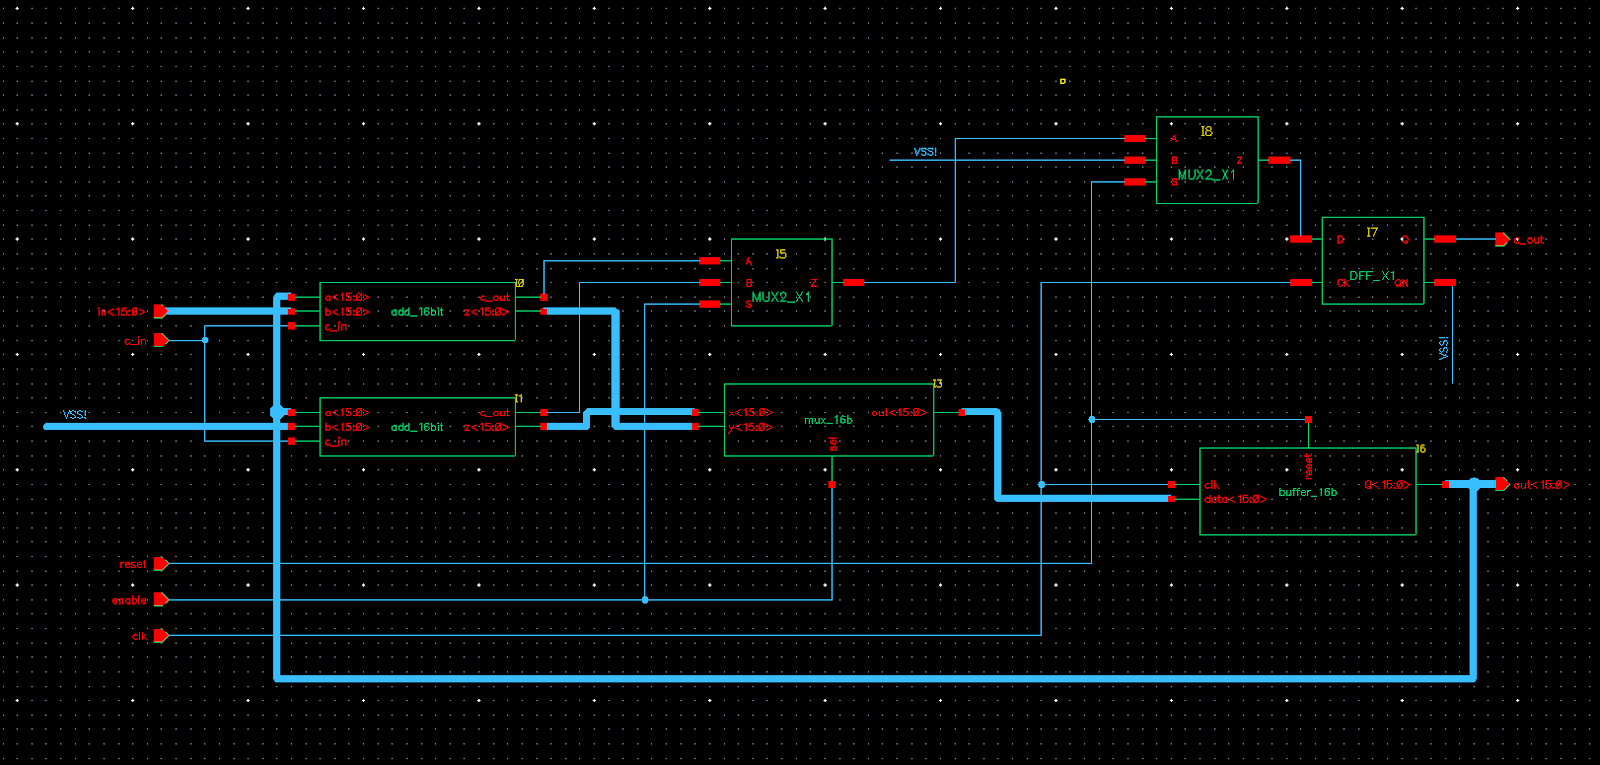
\includegraphics[width=0.85\linewidth]{report_pics/accum16b_schem.png}
		\caption{16-bit accumulator schematic design in Cadence}
		\label{fig7}
	\end{figure}
	
	
	\subsubsection{8-bit comparator}
	The 8-bit comparator is implemented using the add-sub block to subtract input B from input A, yielding a carry-out. If the carry out is 0, the difference between A and B is negative, thus A is less than B. Then, the difference between A and B is checked against 0 to determine if A is equal to B. This is done via a sequence of 7 OR gates to output a logic “1” if equal, then OR-ed with the less-than signal to obtain a less-than-or-equal output signal.
	
	\begin{figure}[htb!]
		\centering
		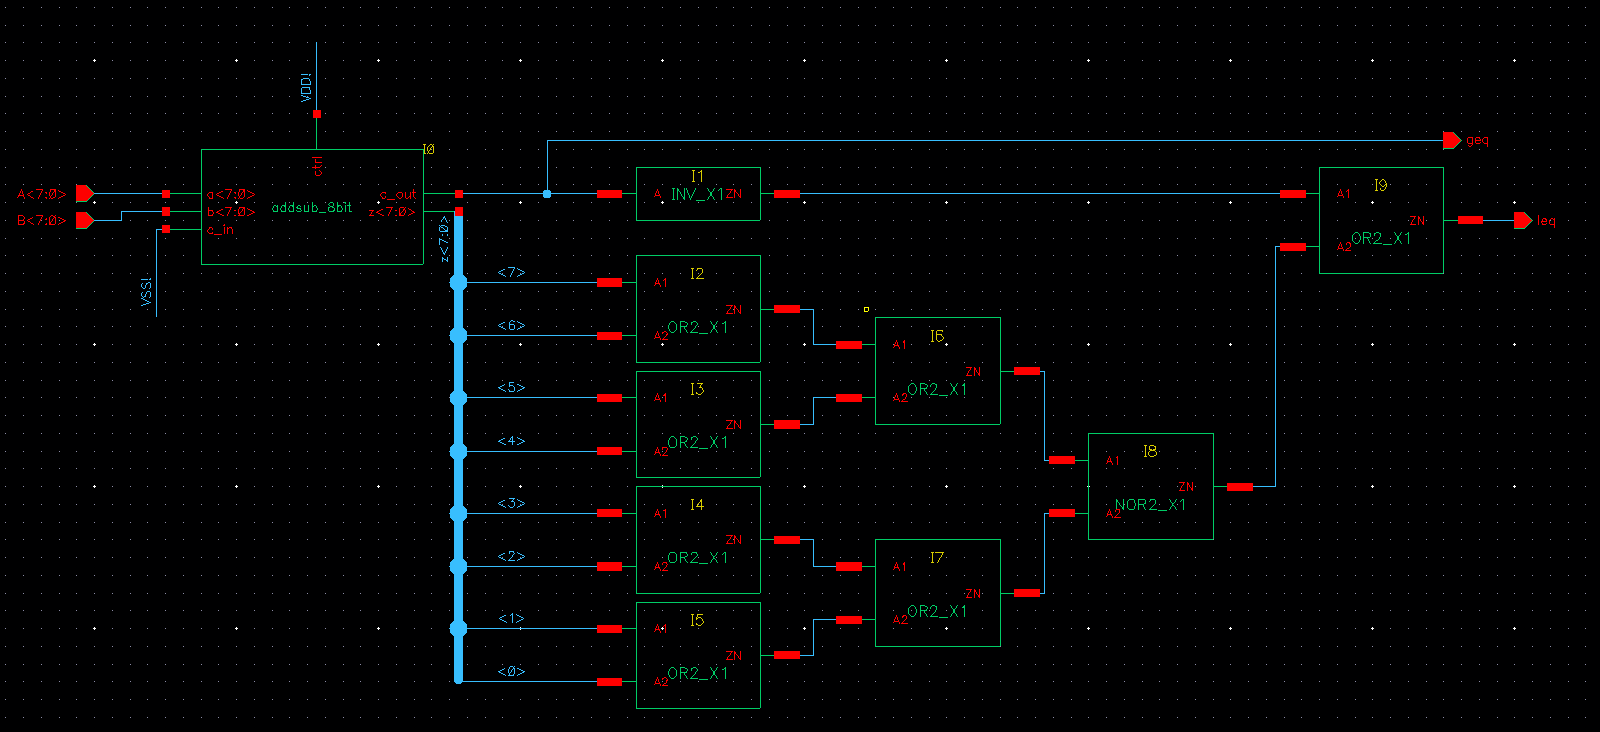
\includegraphics[width=0.85\linewidth]{report_pics/comp8b_schem.png}
		\caption{8-bit comparator schematic design in Cadence}
		\label{fig8}
	\end{figure}
	
	\newpage
	
	\subsubsection{Absolute difference calculation block}
	The absolute difference calculation block calculates $|A - B|$.
	
	\begin{figure}[htb!]
		\centering
		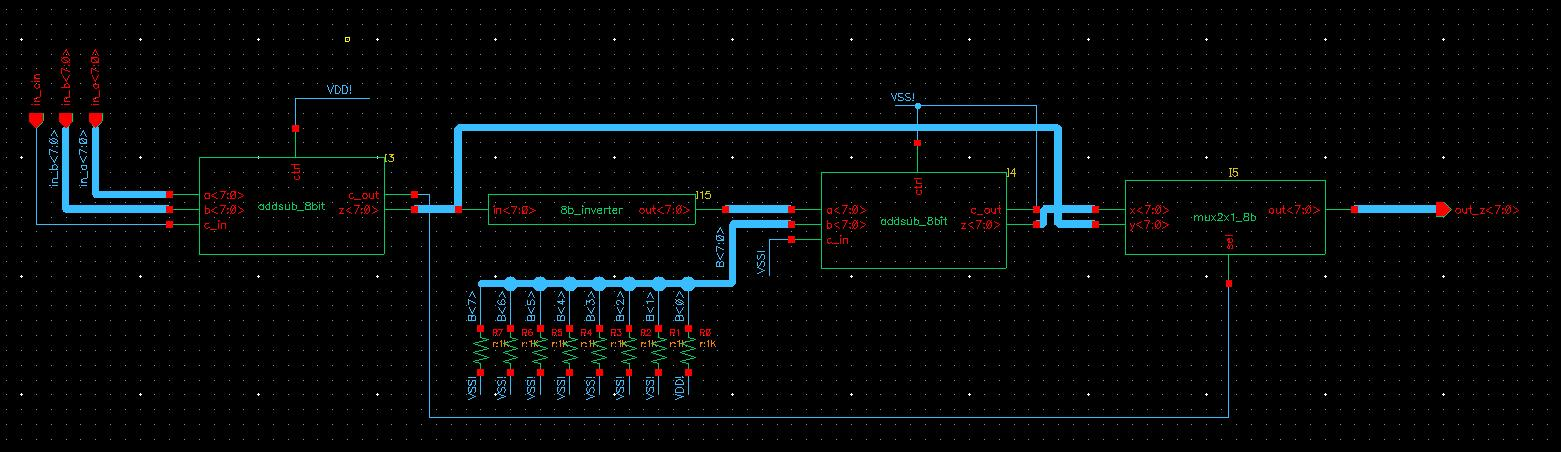
\includegraphics[width=0.85\linewidth]{report_pics/abs_8b_schem.jpg}
		\caption{8-bit absolute difference schematic design in Cadence}
		\label{fig9}
	\end{figure}
	
	
	\subsubsection{Exponential unit}
	Since we are using Taylor series to estimate the exponential function (equation \ref{eq7}), the exponential unit is only made up of 8-bit multipliers and 8-bit adders. In addition, since the function we are trying to calculate is $e^{-x^2}$ (equation \ref{eq6}), we need 3 multipliers to calculate $x^2$, $x^4$, $\frac{1}{2}x^4$, and 2 adder-subtractors to add $1$ to  $- x^2$ then to $ \frac{1}{2}x^4$.
	
	
	\begin{figure}[htb!]
		\centering
		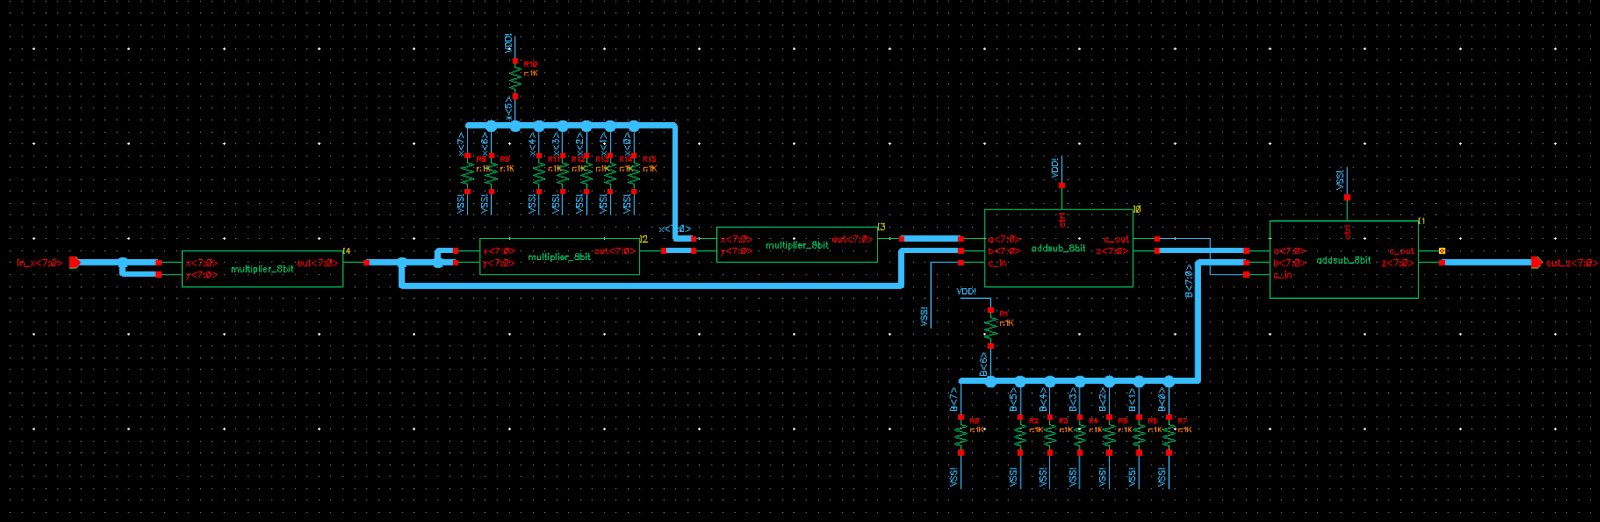
\includegraphics[width=0.85\linewidth]{report_pics/exp8b_schem.png}
		\caption{8-bit exponential unit schematic design in Cadence}
		\label{fig10}
	\end{figure}
	
	\newpage
	
	\subsubsection{Array multiplier}
	The array multiplier is built upon 64 processing elements (pe), which is a 1-bit full adder that also passes on the input bits. As all of the processing elements are wired according to the schematic, a 8x8-bit multiplier is created with the output of 16 bits. The output, however, can be re-wired to fit with the interpretation of fixed-point real number. For example, we want to multiply 2 2Q6 numbers to get another 2Q6 number, then we can drop the first 2 bits and the last 6 bits. This is because when multiplying a 2Q6 with a 2Q6 number, a usual output should be 4Q12, in which the decimal dot is interpreted to be placed between bit 12 and bit 11. To obtain a 2Q6 output, we discard the first 2 bits and the last 6 bits. There is a also different circumstance where we multiply a 8Q0 number with a 0Q8 number and expect a 4Q4 number as the output. Here, we drop the first 4 bits and the last 4 bits to get the desired result.
	
	\begin{figure}[htb!]
		\centering
		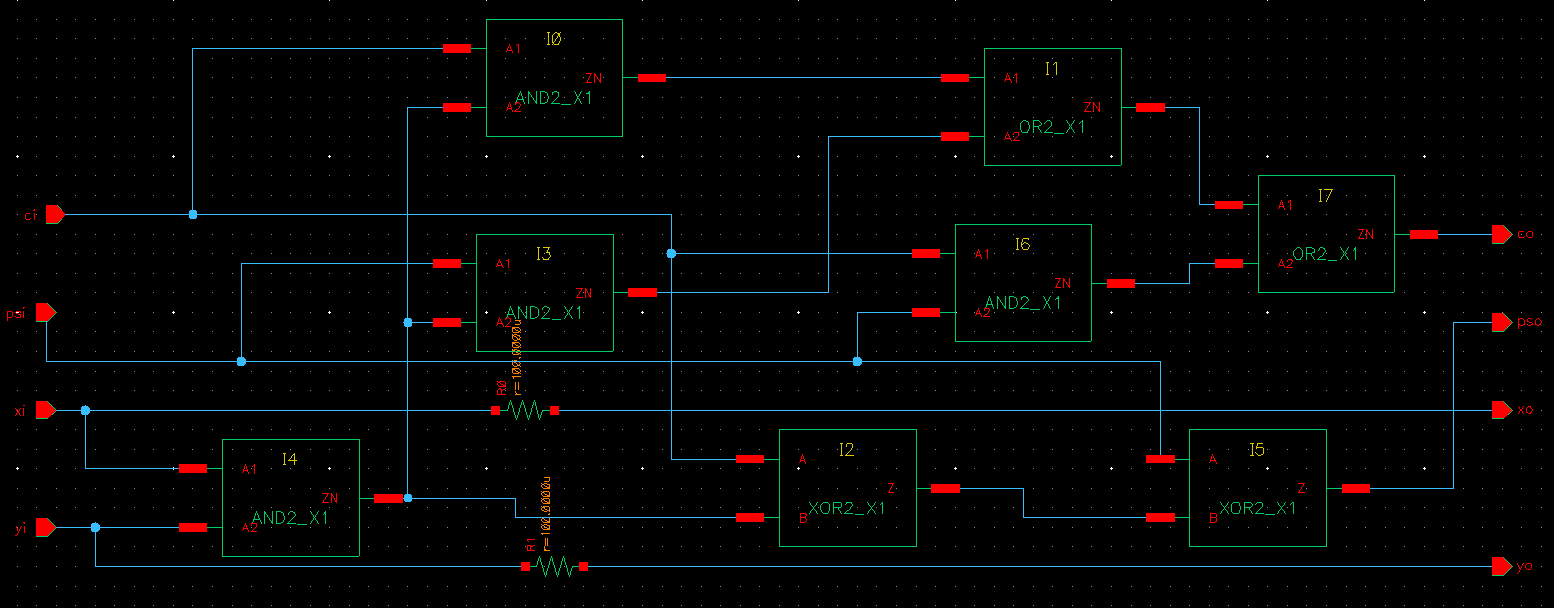
\includegraphics[width=0.85\linewidth]{report_pics/arr_mult_pe_schem.png}
		\caption{PE of array multiplier schematic design in Cadence}
		\label{fig11}
	\end{figure}
	
	\newpage
	
	\subsubsubsection{8-to-16 bit array multiplier}
	
	\begin{figure}[htb!]
		\centering
		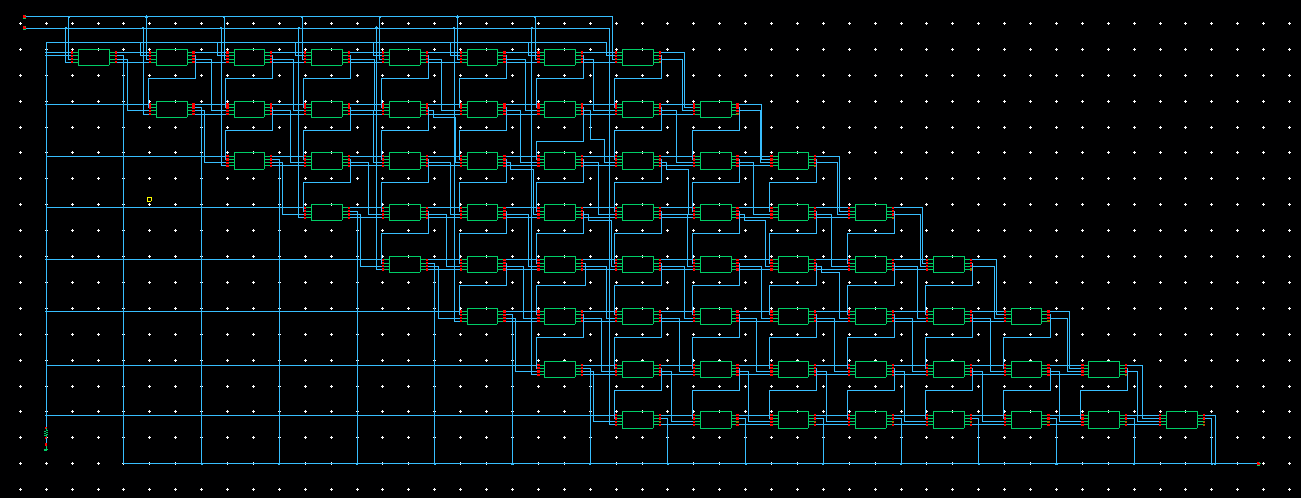
\includegraphics[width=0.85\linewidth]{report_pics/8to16_mult_schem.png}
		\caption{8-to-16 bit array multiplier schematic design in Cadence}
		\label{fig12}
	\end{figure}
	
	\subsubsubsection{8-to-8 bit array multiplier}
	
	\begin{figure}[htb!]
		\centering
		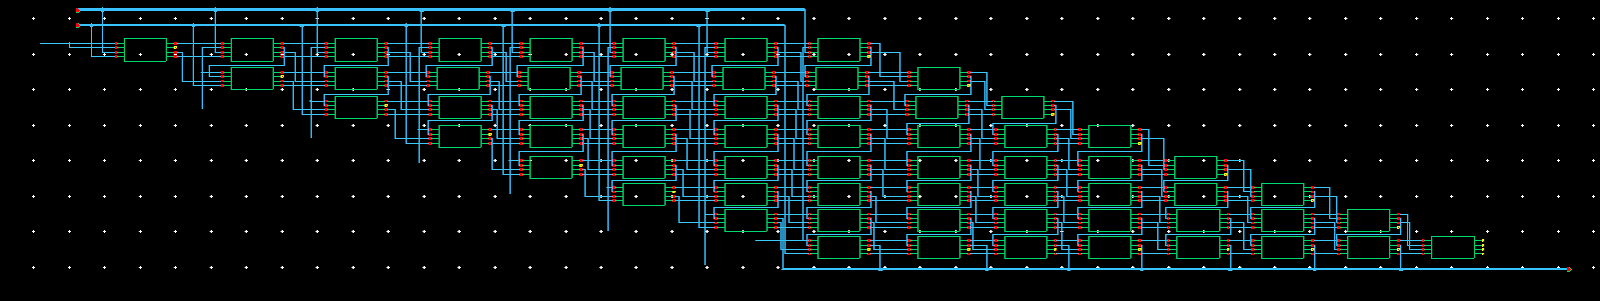
\includegraphics[width=0.85\linewidth]{report_pics/8to8_mult_schem.png}
		\caption{8-to-8 bit array multiplier schematic design in Cadence}
		\label{fig13}
	\end{figure}
	
	\subsubsection{8-bit array divider}
	Our implementation of the combinational array divider has 8 processing elements for producing 8 bits, each of which consists of an 8-bit adder, a comparator and a MUX. Within each of these elemental units, the dividend X is shifted, subtracted and compared with divisor Y to set the according bit of the quotient. The remainder of the division is the leftover of the last unit. The divider will output both the quotient and the remainder as 2 8-bit numbers. This design is inspired by a paper by Narendra, 2015 \cite{6}.
	
	\begin{figure}[htb!]
		\centering
		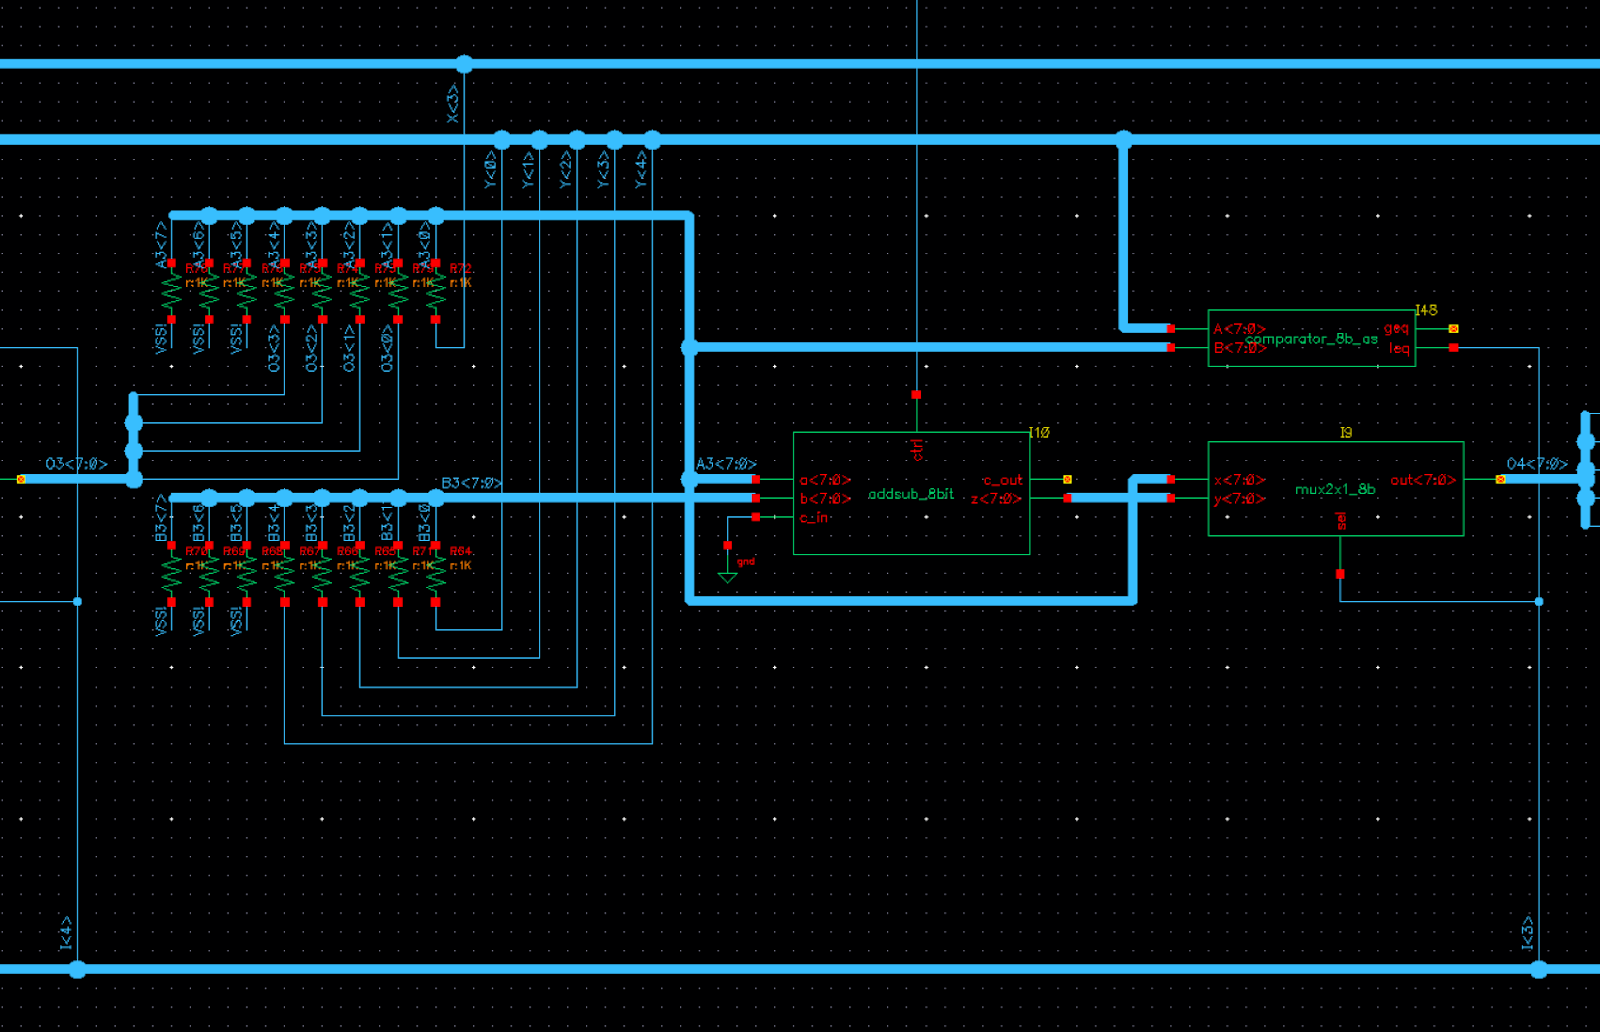
\includegraphics[width=0.85\linewidth]{report_pics/arr_div_pe_schem.png}
		\caption{Array divider's PE schematic design in Cadence}
		\label{fig14}
	\end{figure}
	
	\begin{figure}[htb!]
		\centering
		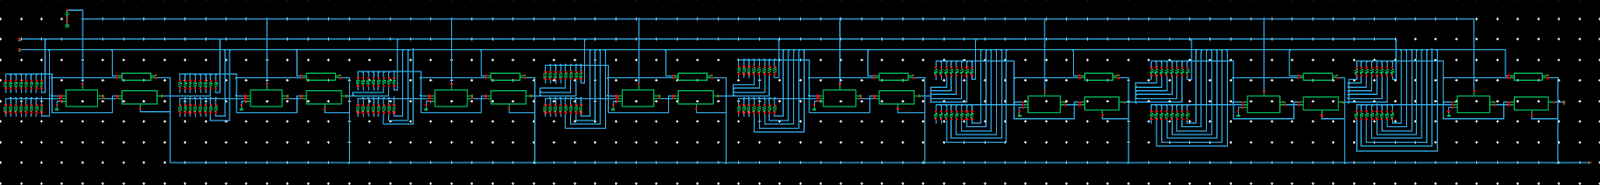
\includegraphics[width=0.85\linewidth]{report_pics/div8b_schem.png}
		\caption{8 bit array divider schematic design in Cadence}
		\label{fig15}
	\end{figure}
	
	\newpage
	\subsection{Memory Blocks}
	\label{subsec:mem}
	
	\subsubsection{16-bit DFF-based register}
	This buffer is set to 0x0000 whenever reset goes to high. Otherwise, the functionality of this buffer is the same as a DFF.
	
	\begin{figure}[htb!]
		\centering
		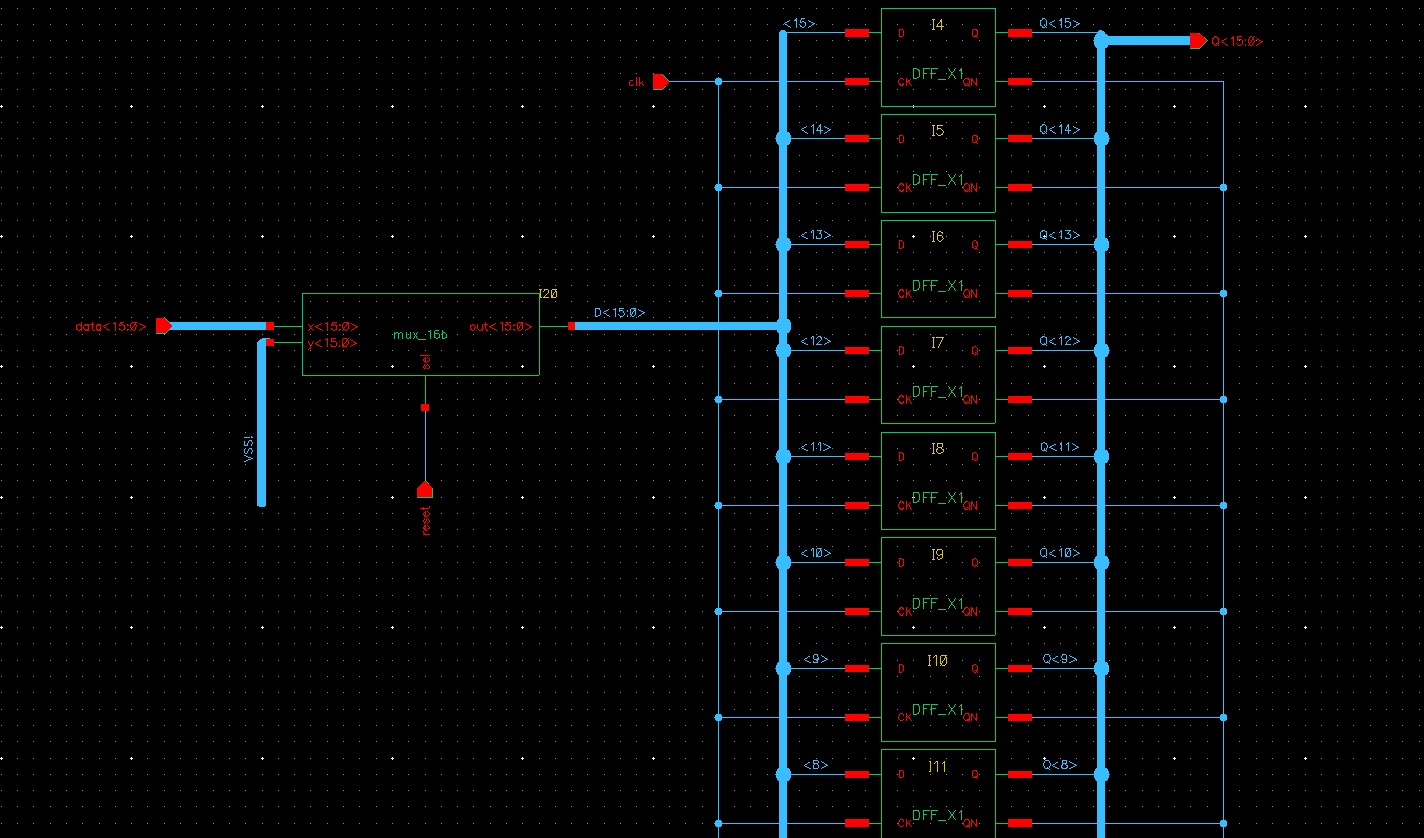
\includegraphics[width=0.85\linewidth]{report_pics/16b_dff_schematic.png}
		\caption{16-bit DFF schematic design in Cadence}
		\label{fig16}
	\end{figure}
	
	\newpage
	
	\subsubsection{8x8 8-bit DFF-based memory}
	For storing the 8x8 blocks of pixels from the input image \textit{I} and the input watermark \textit{W}, we use a 64x8-bit DFF-based memory to store each 8x8 block. Since each value of the grayscale pixel is 8 bits, the memory is byte-addressable by design. Each DFF stores 1 bit and a group of 8 DFF is then called a memory row. To address these rows, a 6-to-64 decoder is implemented.
	
	\subsubsubsection{6-to-64 decoder}
	The 6-to-64 decoder is used to direct write and read data to the corresponding memory row address where the data is desired to be written to or read from.
	
	\begin{figure}[htb!]
		\centering
		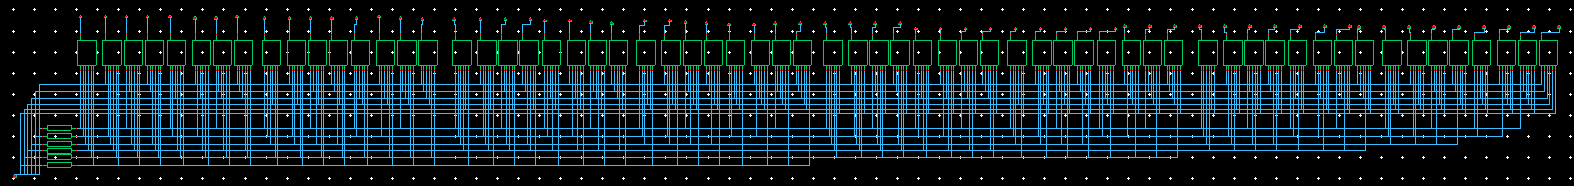
\includegraphics[width=0.85\linewidth]{report_pics/6x64_decoder_schem.png}
		\caption{Schematic of a 6-to-64 decoder that takes in a 6-bit address and turns 1 of its 64 output signals to high, while leaving the rest as low}
		\label{fig17}
	\end{figure}
	
	\begin{figure}[htb!]
		\centering
		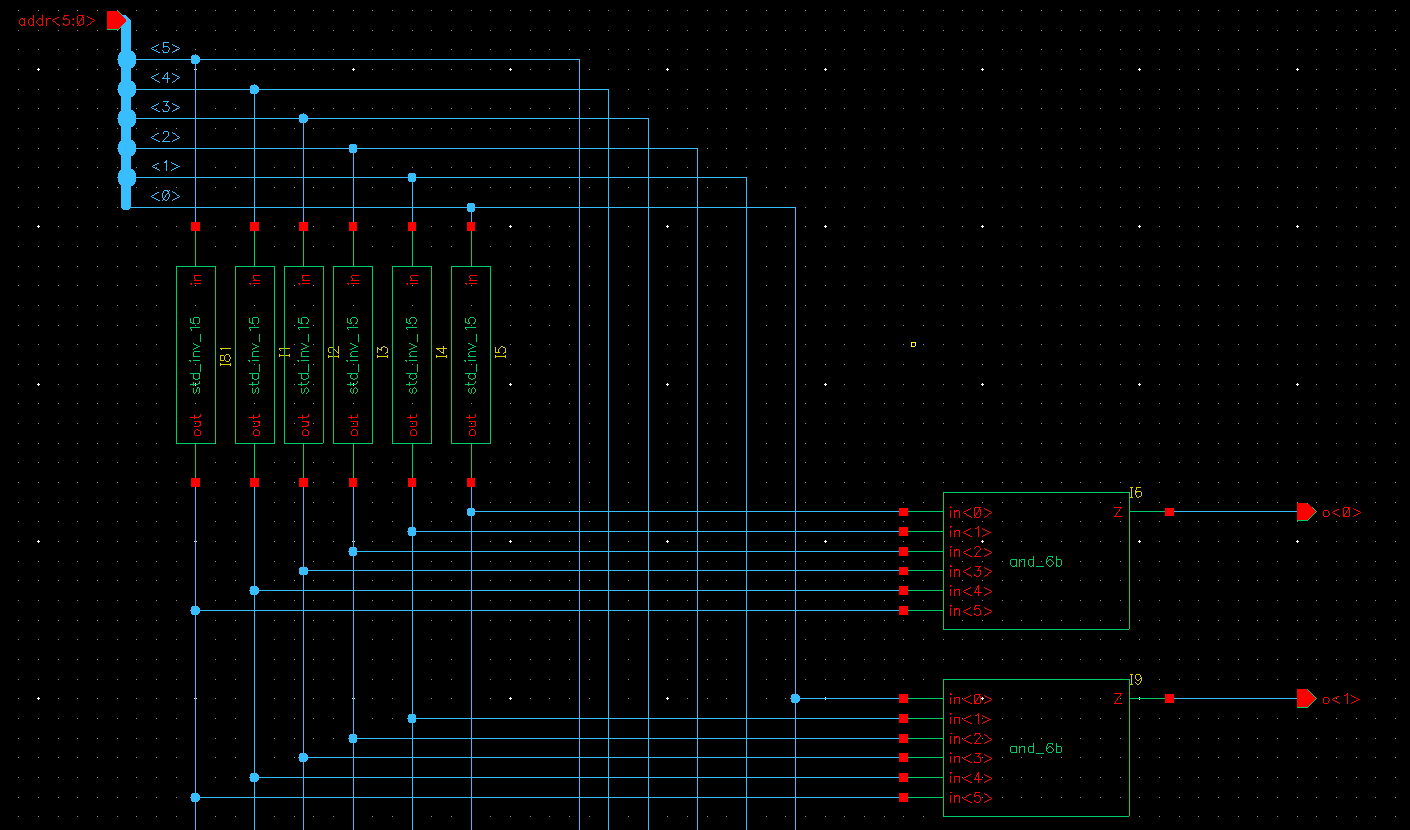
\includegraphics[width=0.85\linewidth]{report_pics/6x64_decoder_detailed.png}
		\caption{Detailed look of the decoder}
		\label{fig18}
	\end{figure}
	
	\subsubsubsection{Read-write enable helper block}
	The desired behavior of a memory cell is to output high impedance (disconnected from the output) when it is not addressed, thus reducing power consumption. Therefore, a helper block to translate the read, write and enable block into only read or write is implemented as above
	
	\begin{figure}[htb!]
		\centering
		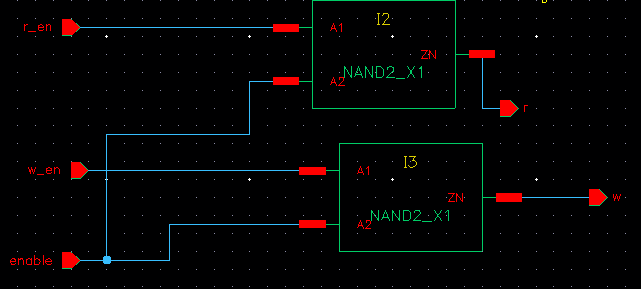
\includegraphics[width=0.85\linewidth]{report_pics/rw_en_helper_schem.png}
		\caption{Read-write enable helper schematic design in Cadence}
		\label{fig19}
	\end{figure}
	
	\subsubsubsection{Memory Cell}
	The memory cell is constructed below in Figure 20 with DFF as the value storing element and a few tri-state buffers for disconnecting from output if not read, disconnecting from input data if not written. The design reasons are discussed in section \ref{sec:specs}.
	
	\begin{figure}[htb!]
		\centering
		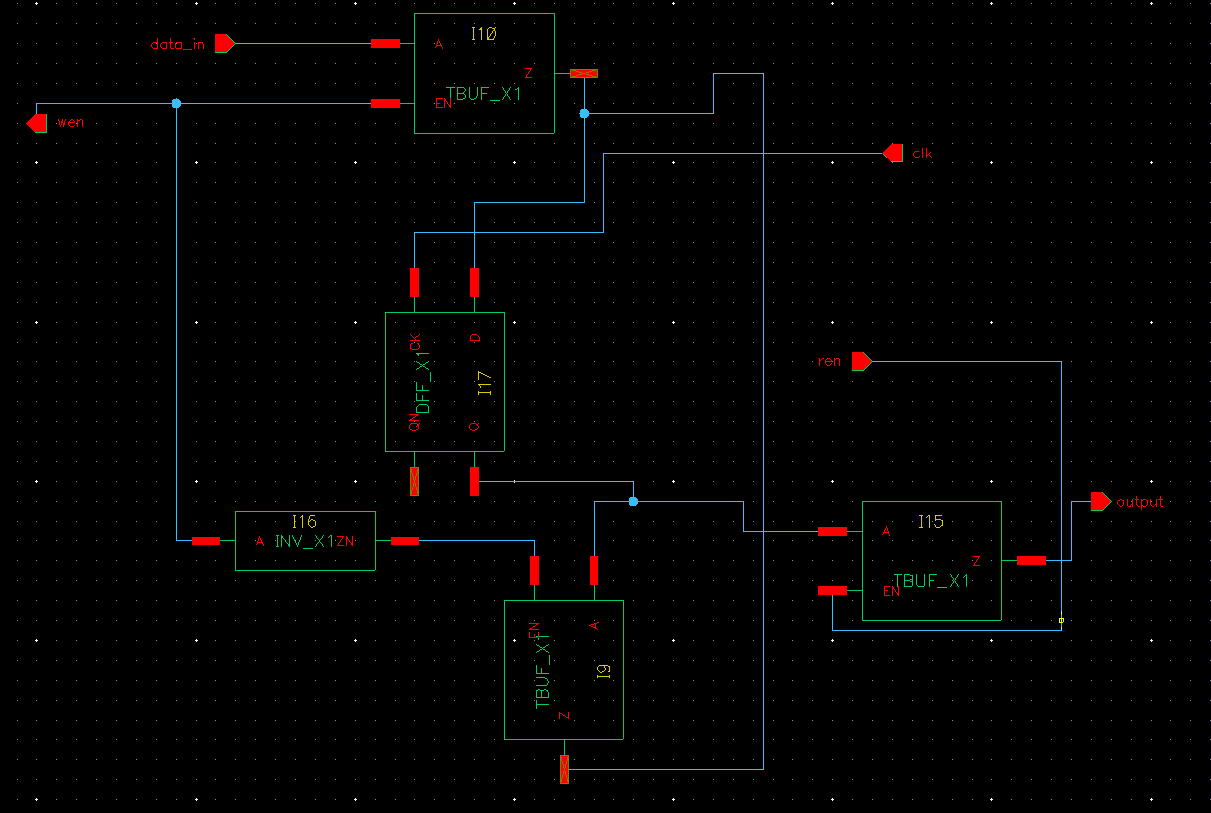
\includegraphics[width=0.85\linewidth]{report_pics/mem_cell_schem.png}
		\caption{Memory Cell schematic design in Cadence}
		\label{fig20}
	\end{figure}
	
	\subsubsubsection{Memory Row}
	A memory row can store 8-bit, the number of bits needed to store any value of a grayscale pixel. These rows are modularized into a package called mem\_row with all the required control data: read, write, enable and clock. The memory row makes use of the read-write enable helper block and 8 memory cells.
	
	\begin{figure}[htb!]
		\centering
		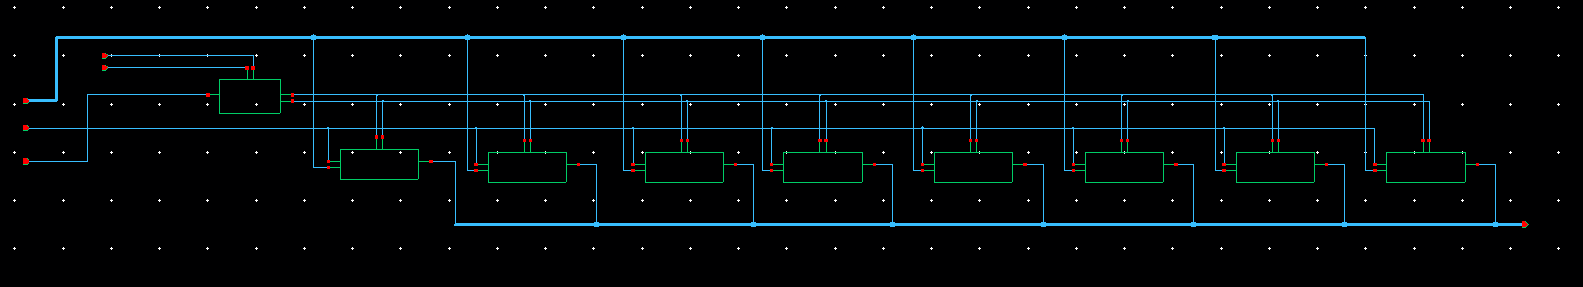
\includegraphics[width=0.85\linewidth]{report_pics/mem_row_schem.png}
		\caption{Memory Row schematic design in Cadence}
		\label{fig21}
	\end{figure}
	
	\subsubsubsection{The 8x8 memory block}
	The structure of the memory is displayed in Figure 22 below. In the memory block, there is a 6-to-64 decoder to address 1 of the 64 mem\_rows at a time, and the control signals as well as input data for writing are wired to every row. Although these are wired, they do not necessarily drive a load of 64 rows thanks to the tri-state buffers that are implemented in each cell which disconnect the data\_in signal from the DFF when the write control signal is low.
	
	\begin{figure}[htb!]
		\centering
		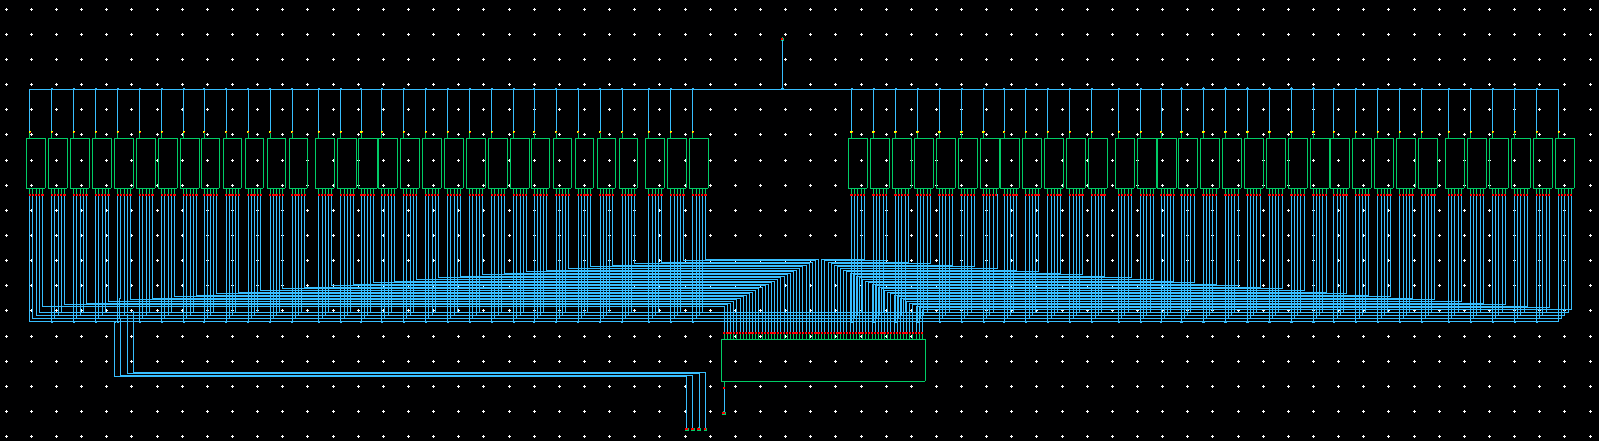
\includegraphics[width=0.85\linewidth]{report_pics/mem_block_schem.png}
		\caption{64 memory rows schematic design in Cadence}
		\label{fig22}
	\end{figure}
	
	\begin{figure}[htb!]
		\centering
		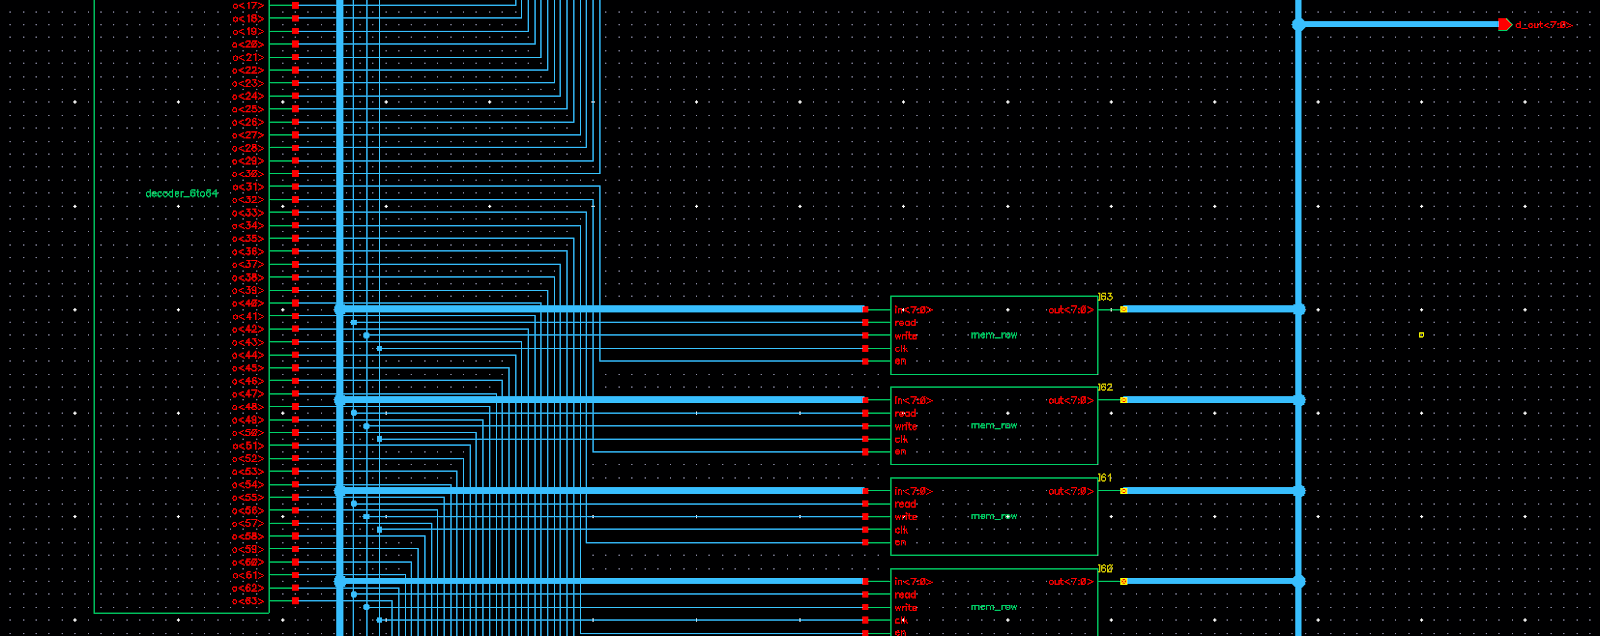
\includegraphics[width=0.85\linewidth]{report_pics/mem_block_detailed.png}
		\caption{A closer look at the memory rows design in Cadence}
		\label{fig23}
	\end{figure}
	
	\subsection{Edge Detection Unit}
	\label{subsec:edge_detect}
	
	The edge detection block comprises 2 absolute differences block to obtain the vertical $Gv(m, n)$ and horizontal gradient $Gh(m, n)$ of each pixel. The horizontal and vertical gradients are then added together and accumulated. The accumulated sum is then averaged (over 64 pixels accumulated) and compared with a user-input threshold. In our implementation of the edge detection block, most smaller units are kept similar with the diagram proposed in the paper in Figure 2(b) except for the multiplier with constant input of 64, used for averaging the gradient cumulative sum. As the multiplication for averaging is the same as shifting the gradient cumulative sum by 6 bits, only bits 13:6 are wired to the input of the next block, the comparator. This bit mapping can be seen in the schematic shown in the below figure.
	
	\begin{figure}[htb!]
		\centering
		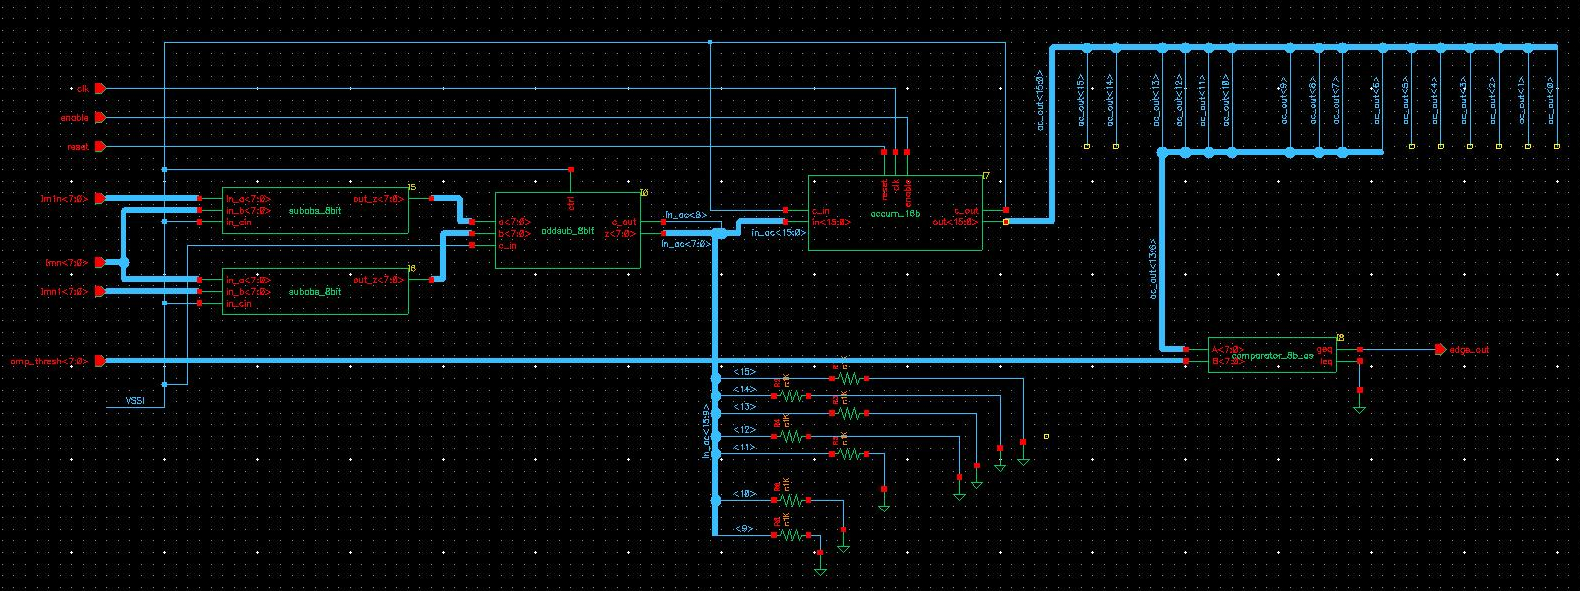
\includegraphics[width=0.85\linewidth]{report_pics/edge_detect_schem.jpg}
		\caption{Edge Detection Unit schematic design in Cadence}
		\label{fig24}
	\end{figure}
	
	\subsection{$\alpha_k$ and $\beta_k$ Calculation Unit}
	\label{subsec:akbk}
	
	The alpha beta calculation takes in the pixel one by one, but only outputs the alpha and beta values when it has finished loading in and computing on all pixels in a 8x8 block. The reason for this is to calculate the local statistics of the 8x8 blocks, including the mean and standard deviation values.
	
	The alpha-beta calculation unit can be divided into 2 main logic paths. One is to output the alpha value and one is to output the beta value. 
	
	On the alpha path, the mean value of the block is calculated by accumulating the input pixel value using the 16-bit accumulator, padding 0s to the 8 MSBs of the accumulator input. The output of the accumulator is then normalized by dividing by $2^{14} (= 16384)$, which is the maximum value that can be accumulated, equals to 64x256. This normalized mean is $\mu_{kI}$ as in the referenced paper [1]. In our implementation, instead of using the array  multiplier to multiply the cumulative sum of input values, we then “shifted” the sum only by discarding some bits of the less significant bits as we recognize that the dividend is an exponential of 2. 
	
	Note that, all real number values in this design are interpreted in the 2Q6 format, which is 2 bit for the integer part, while the 6 LSBs are for the decimal part. Therefore, in order to preserve the most decimal bits after dividing by 16384, the signal's 8 LSB is discarded, and the 8 MSB are interpreted as 2Q6.
	
	The alpha part continues to subtract 0.5, (hard wired in our implementation) to get the absolute difference between the normalized mean and the mean grey value of an average image. This difference is then input into the exponential unit, then divided by the standard deviation of the block, and fitted into the range of alpha max and min to get the alpha value.
	
	The beta path is implemented similar to the block diagram in Figure 2a. Similar to the alpha path, all the constants are hard wired, and the divisions with power of 2 dividends are done with bit mapping instead of multipliers.
	
	
	\begin{figure}[ht!]
		\centering
		\begin{subfigure}[b]{.558\linewidth}
			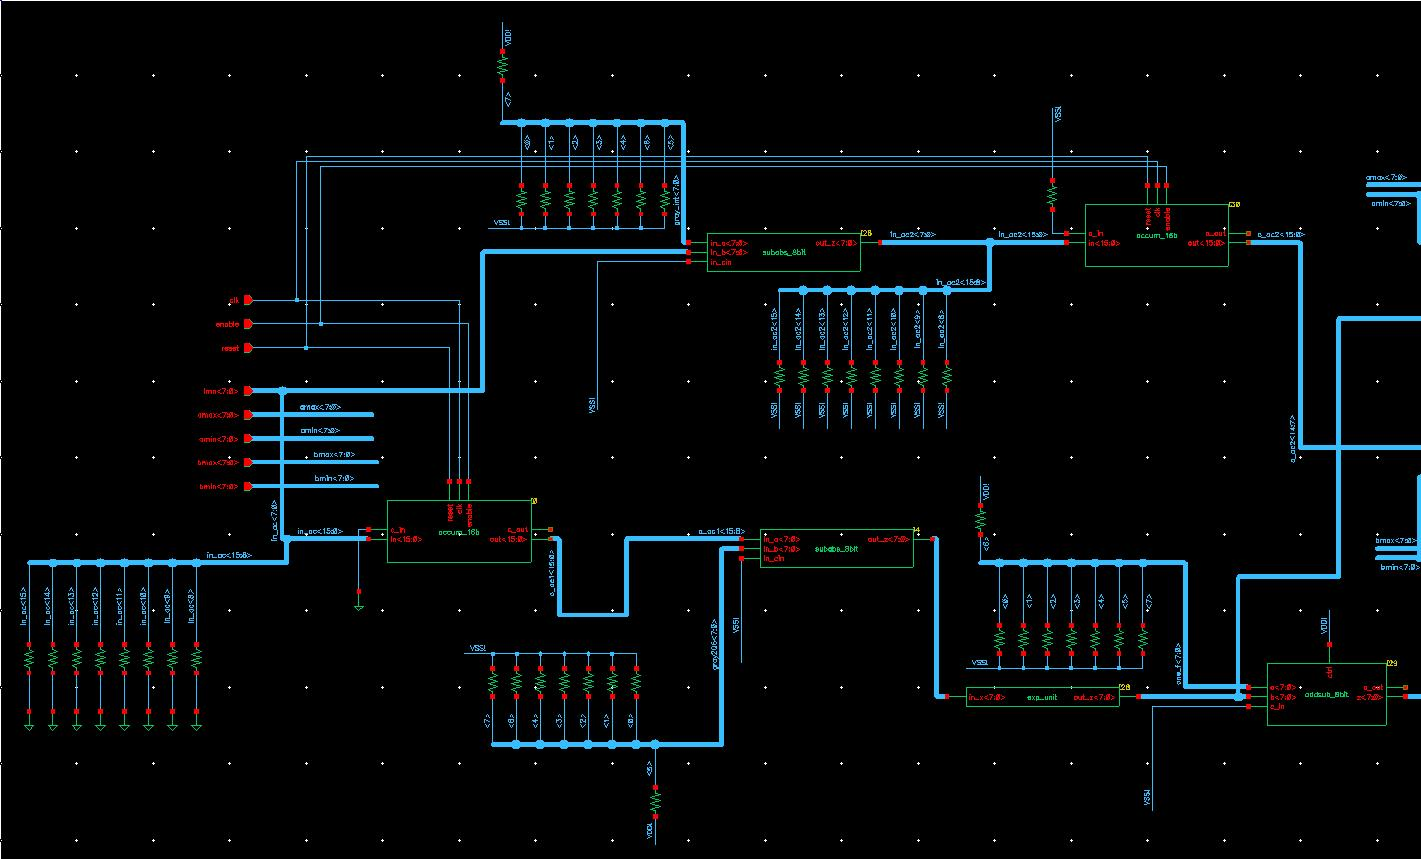
\includegraphics[width=\textwidth]{report_pics/ak_bk_left.jpg}
			\caption{}
			\label{fig25a}
		\end{subfigure}
		\begin{subfigure}[b]{.4\linewidth}
			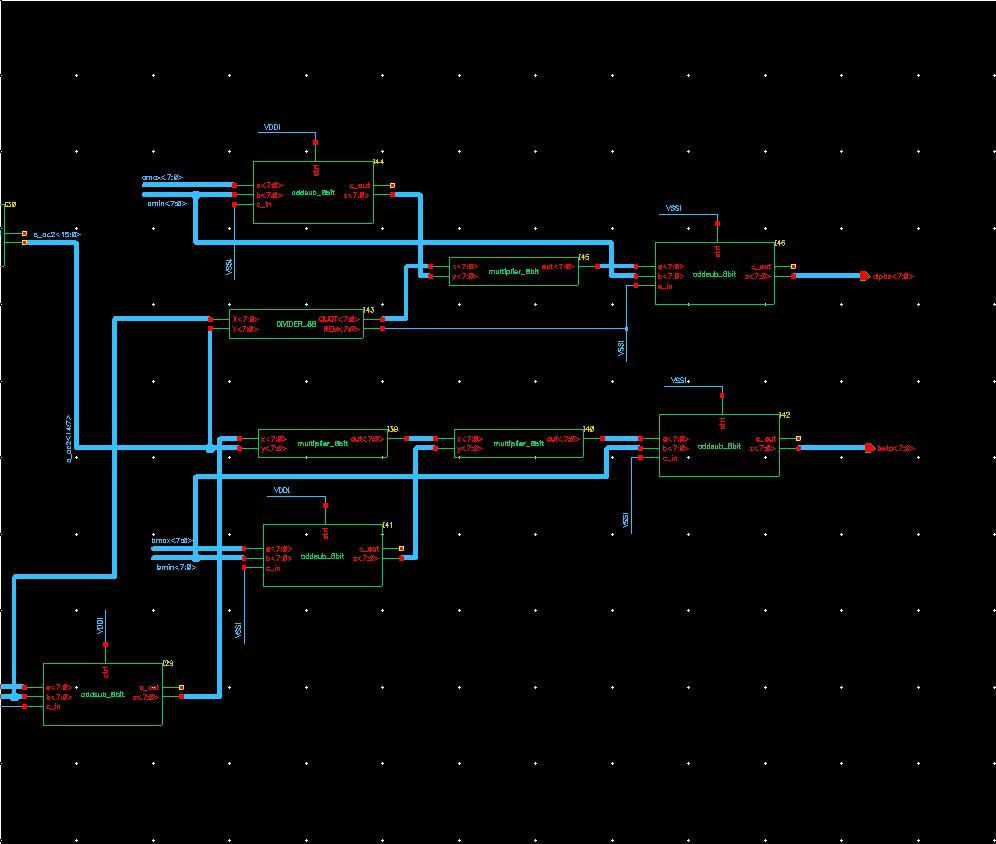
\includegraphics[width=\textwidth]{report_pics/ak_bk_right.jpg}
			\caption{}
			\label{fig25b}
		\end{subfigure}
		\caption{(a) Left and (b) Right side of the $\alpha_k$ and $\beta_k$ Calculation Unit}
	\end{figure}
	\newpage
	\subsection{Overall Datapath}
	\label{subsec:datapath}
	
	As core logic intermediate blocks are designed, they are connected within the datapath network to map the inputs into the component blocks to produce the final output. Although the results of alpha - beta unit are fixed-point real numbers in 2Q6 format, it is necessary to transform them into 0Q8 format to maintain coherence with values from register files and scaling factor ($a_i$). Therefore, the output of the first two MUX is re-wired to eliminate first two bits and pad two zero bits at the end to accomplish this purpose. Then, each of the first two multipliers takes one input in 0Q8 format and another in 8Q0 format to produce an output in 8Q8 format. At this point, if the chosen algorithm is the first one, the middle 8 bits of each output of the multipliers are passed into the last multiplier, and the output of this multiplier is also in 8Q8 format. After that, the first 8 bits are mapped to the MUX and adder to produce the output for algorithm 1. On the other hand, if algorithm 2 is selected, the first 8 bits of each result is mapped to two MUXs and then added to get the final result.
	
	
	\begin{figure}[ht!]
		\centering
		\begin{subfigure}[b]{.411\linewidth}
			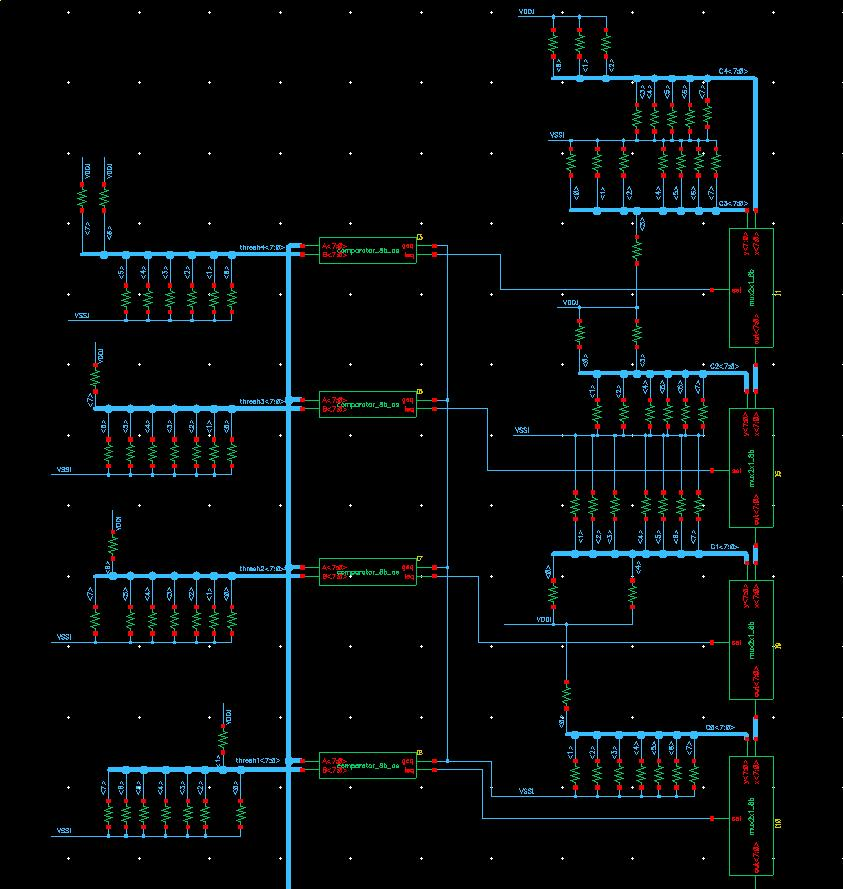
\includegraphics[width=\textwidth]{report_pics/datapath_top.jpg}   
			\caption{}
			\label{fig26a}
		\end{subfigure}
		\\
		\begin{subfigure}[b]{.4\linewidth}
			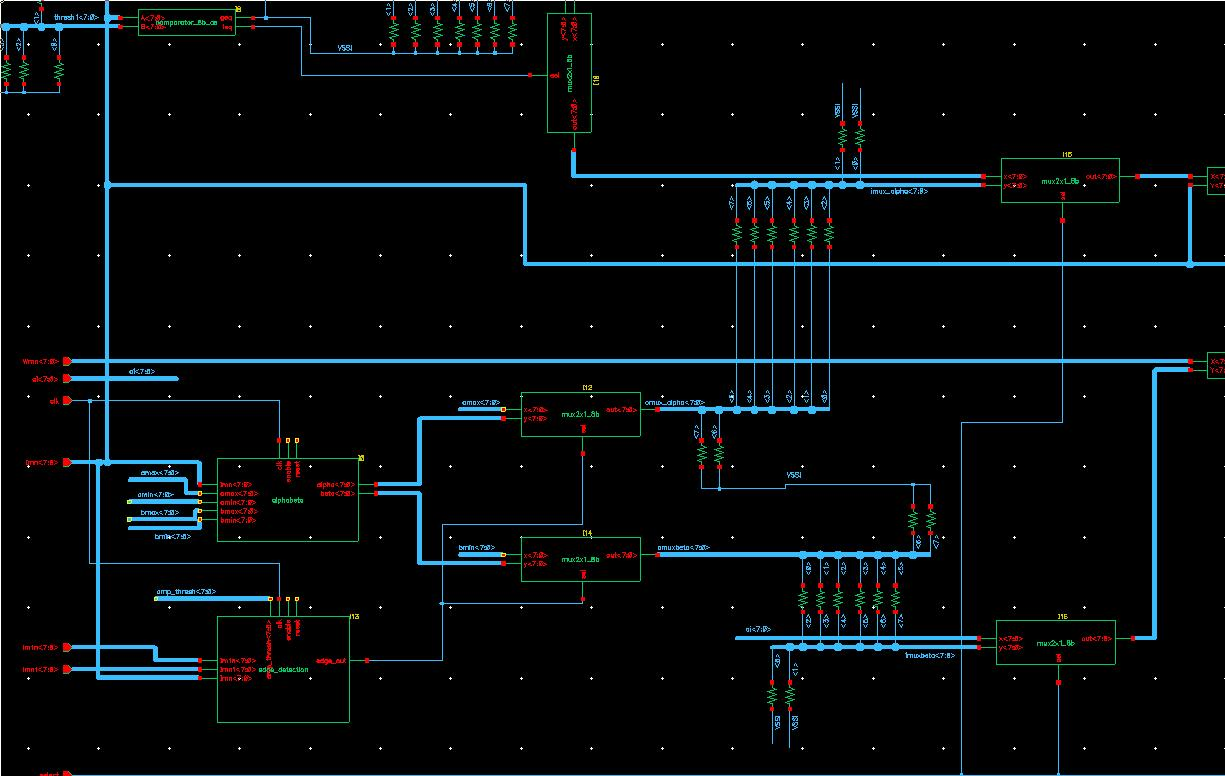
\includegraphics[width=\textwidth]{report_pics/datapath_btm_left.jpg}
			\caption{}
			\label{fig26b}
		\end{subfigure}
		\begin{subfigure}[b]{.4\linewidth}
			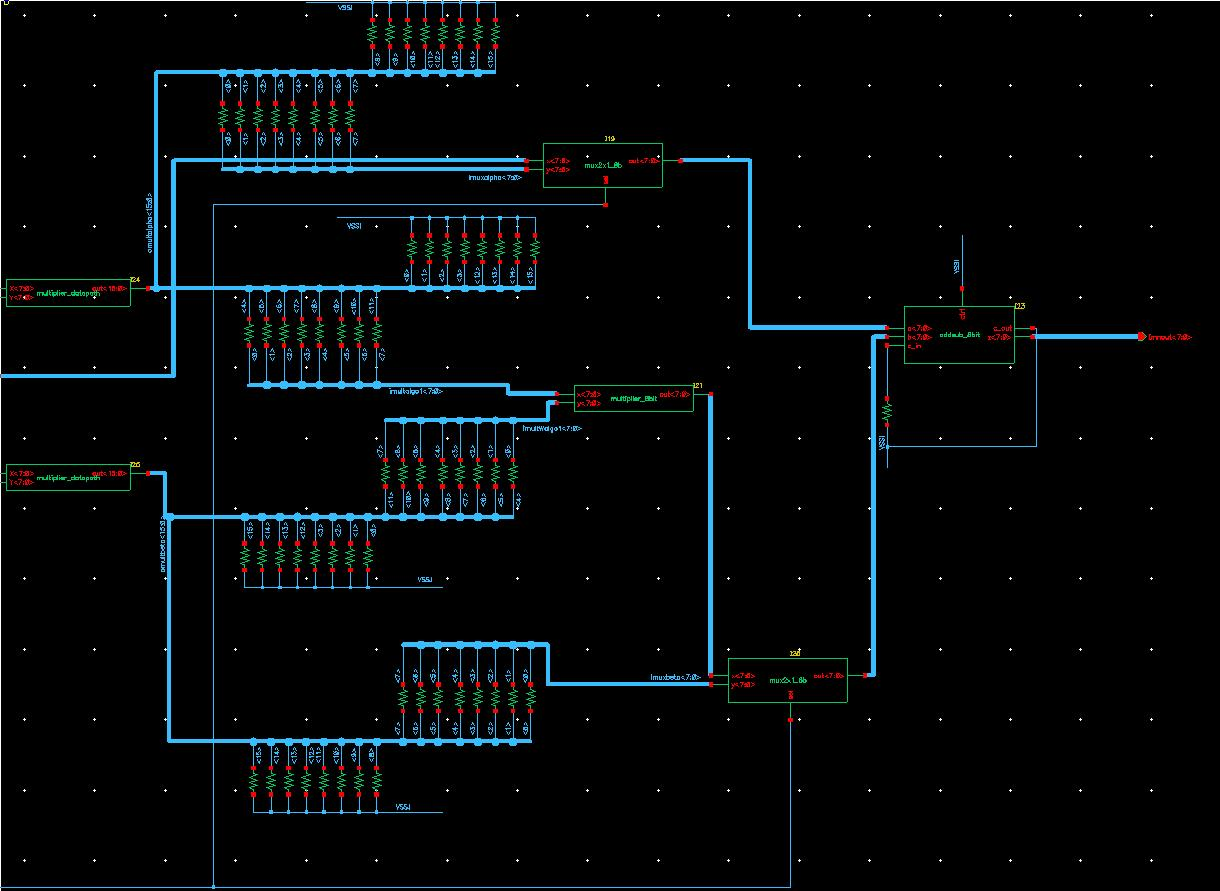
\includegraphics[width=\textwidth]{report_pics/datapath_btm_right.jpg}
			\caption{}
			\label{fig26c}
		\end{subfigure}
		\caption{(a) Top, (b) Left, and (c) Right side of the Overall Datapath}
	\end{figure}
	
	\newpage
	\subsection{Controller and Processor}
	\label{subsec:controller}
	
	\subsubsection{Finite State Machine}
	The controller is responsible for propagating data into the datapath based on two control signals “start” and “select”. The controller waits for the “start” signal to initiate the calculation in the datapath. Here, if “select” is 0, the processor will calculate the watermarked image using algorithm 1, and use algorithm 2 for calculations if “select” is 1. In algorithm 1, the processor reads the input pixel, directly performs calculation on that pixel, and outputs the watermarked pixel. In algorithm 2, the processor needs to load an 8x8 pixel block of the original image and an 8x8 pixel block of the watermark image before it can proceed with the calculation. The Read Block state is therefore used to load all the pixels into the two 8x8 memory blocks in the processor. Once reading is finished, the data will then be loaded from the memory blocks into the datapath every clock cycle, and the processor’s output data is directly mapped from the output of the datapath.
	
	\begin{figure}[htb!]
		\centering
		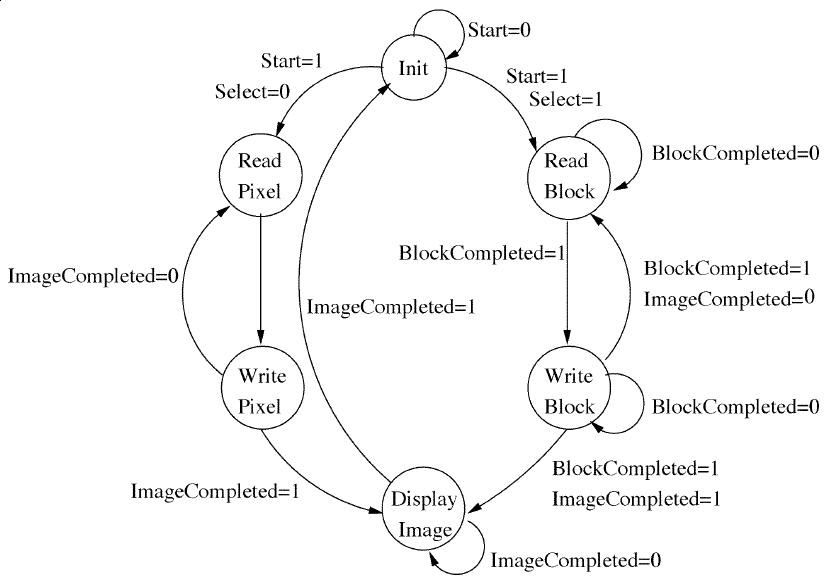
\includegraphics[width=0.85\linewidth]{report_pics/fsm.jpg}
		\caption{High level overview of the controller}
		\label{fig27}
	\end{figure}
	
	\subsubsection{Implementation}
	For ease of implementation, the Read Block state is used for both algorithms 1 and 2. In other words, the processor will load 64 pixels before commencing any work in the datapath. Therefore, in algorithm 1, the total time it takes to finish calculating the first pixel is 64 + 2 (transition from Init state to Read Block state) + 1 (transition to Display Image State) + 1 (send input into the datapath) = 68, but from the second pixel onwards, it only takes 1 clock cycle for each pixel.
	
	For algorithm 2, it also takes 64 clock cycles to read two 8x8 input pixel blocks. However, algorithm 2 requires the use of the edge detection block, which requires input data for pixel I(m, n), I(m + 1, n) and I(m, n + 1). Because the memory block designed for this project only has a single port, the processor needs 3 clock cycles to load data for those 3 pixels. Furthermore, the datapath for algorithm 2 requires the calculation for $\alpha_k$, $\beta_k$ and the edge detection unit to finish before it starts, which takes another 64 clock cycles. Therefore, the time it takes for the processor to output the watermarked pixel for the first input pixel is 64 + 3 (load the first 3 pixels into the edge detection block) + 64 (finish calculation of $\alpha_k$ and $\beta_k$)  + 1 (Display Image State) = 132 cycles.
	
	Below is the pinout of the procesor for references.
	
	\begin{figure}[htb!]
		\centering
		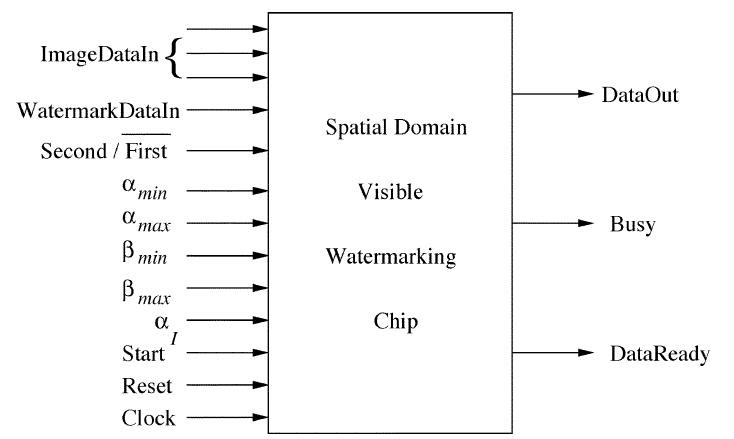
\includegraphics[width=0.85\linewidth]{report_pics/processor_block_diag.jpg}
		\caption{Chip Pinout of the Watermarking Processor}
		\label{fig28}
	\end{figure}
	
	
	\newpage
	
	\section{Testing}
	\label{sec:testing}
	
	In this section, we will present all the testing done on the blocks designed above. The experiments are done using Cadence Virtuoso ADE L Schematic Simulator. The purpose of these experiments is to verify the functionality of the blocks designed above, and gather the timing delay for each of them.
	
	We are denoting the average propagation delay as $t_{avg\_prop}$, and worst case propgation delay as $t_{worst\_prop}$
	
	\subsection{Arithmetic Blocks}
	\label{subsec:arith_blocks}
	
	\subsubsection{8-bit Adder-subtractor}
	
	The figure below (Figure \ref{fig29}) shows our functionality and timing result for the 8-bit Adder-subtractor. The unit performs as expected with $t_{avg\_prop}$ (delay from the moment the input changes to the moment the output changes) of 118.67ps and $t_{worst\_prop} = 131.94ps$.
	
	\begin{figure}[htb!]
		\centering
		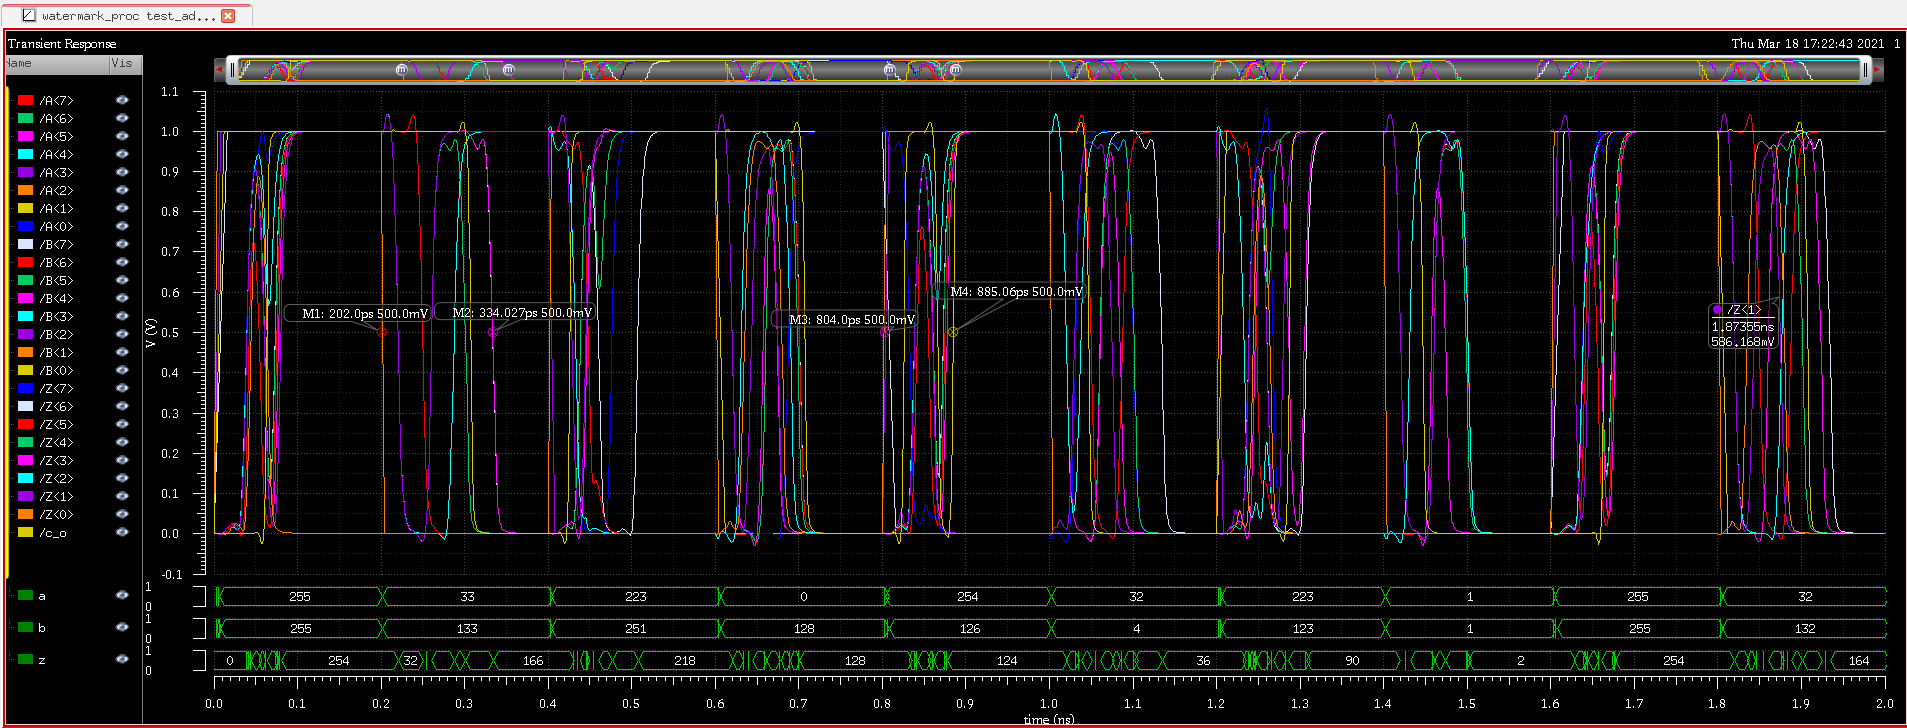
\includegraphics[width=0.85\linewidth]{report_pics/addsub8b_sim.png}
		\caption{Simulation results of the 8-bit Adder-Subtractor}
		\label{fig29}
	\end{figure}
	
	\subsubsection{16-bit Adder}
	
	The figure below (Figure \ref{fig30}) shows our functionality and timing result for the 16-bit Adder. The unit performs as expected with $t_{avg\_prop} = 128.67ps$ and $t_{worst\_prop} = 153.95ps$ 
	
	\begin{figure}[htb!]
		\centering
		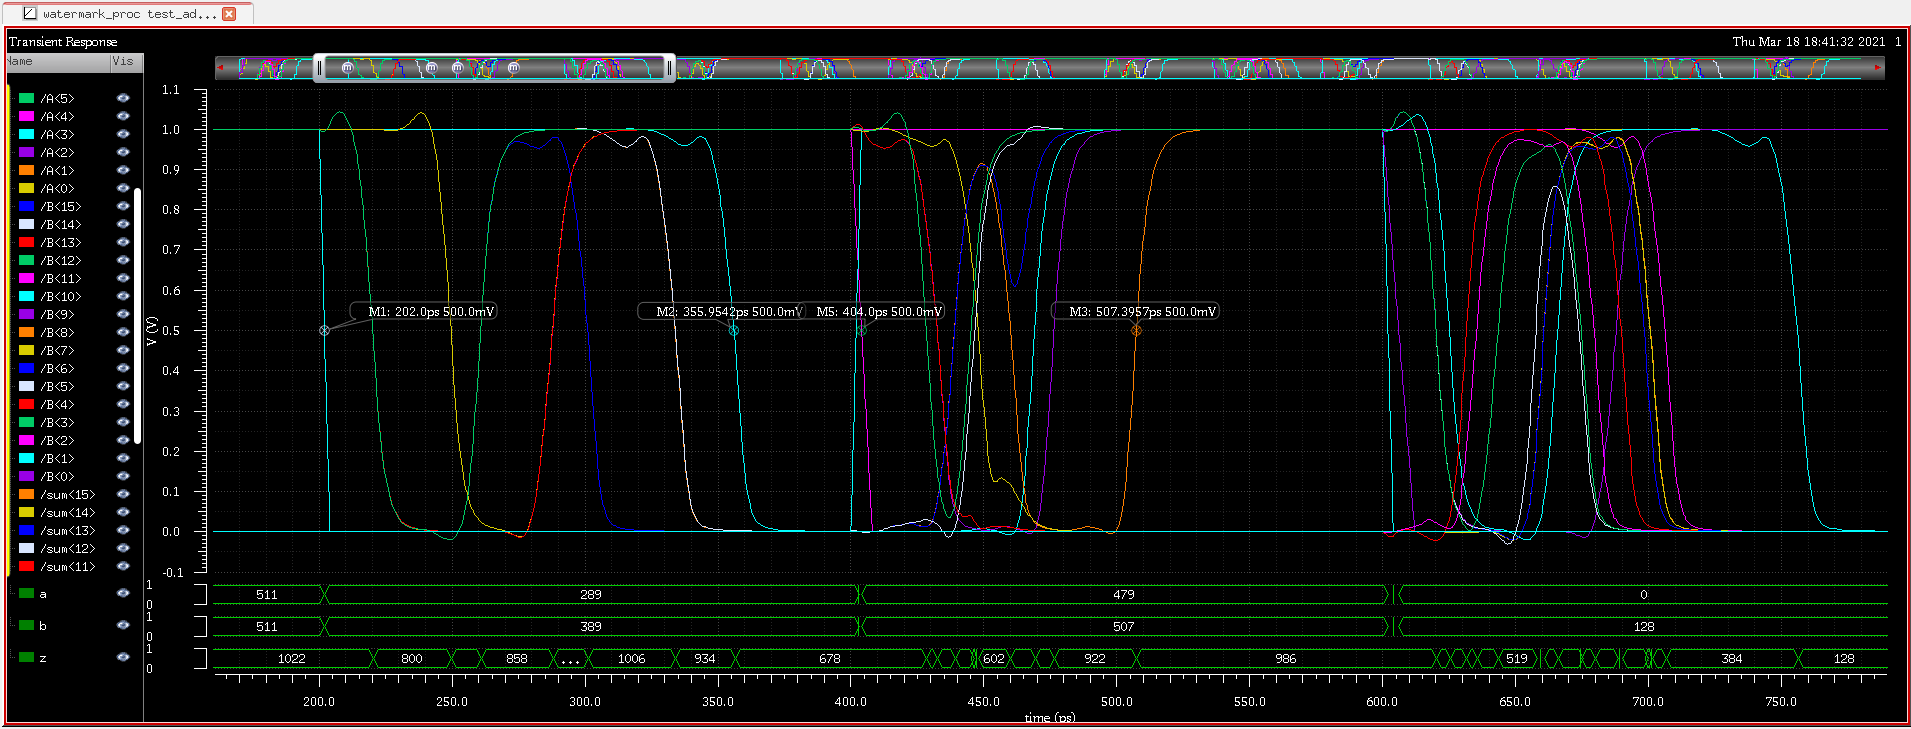
\includegraphics[width=0.85\linewidth]{report_pics/add16b_sim.png}
		\caption{Simulation results of the 16-bit Adder}
		\label{fig30}
	\end{figure}
	
	
	\subsubsection{16-bit Accumulator}
	
	The figure below (Figure \ref{fig31}) shows our functionality and timing result for the 16-bit Accumulator. The unit performs as expected with $t_{avg\_prop} = 42.11ps$  and $t_{worst\_prop} = 44.04ps$. 
	
	\begin{figure}[htb!]
		\centering
		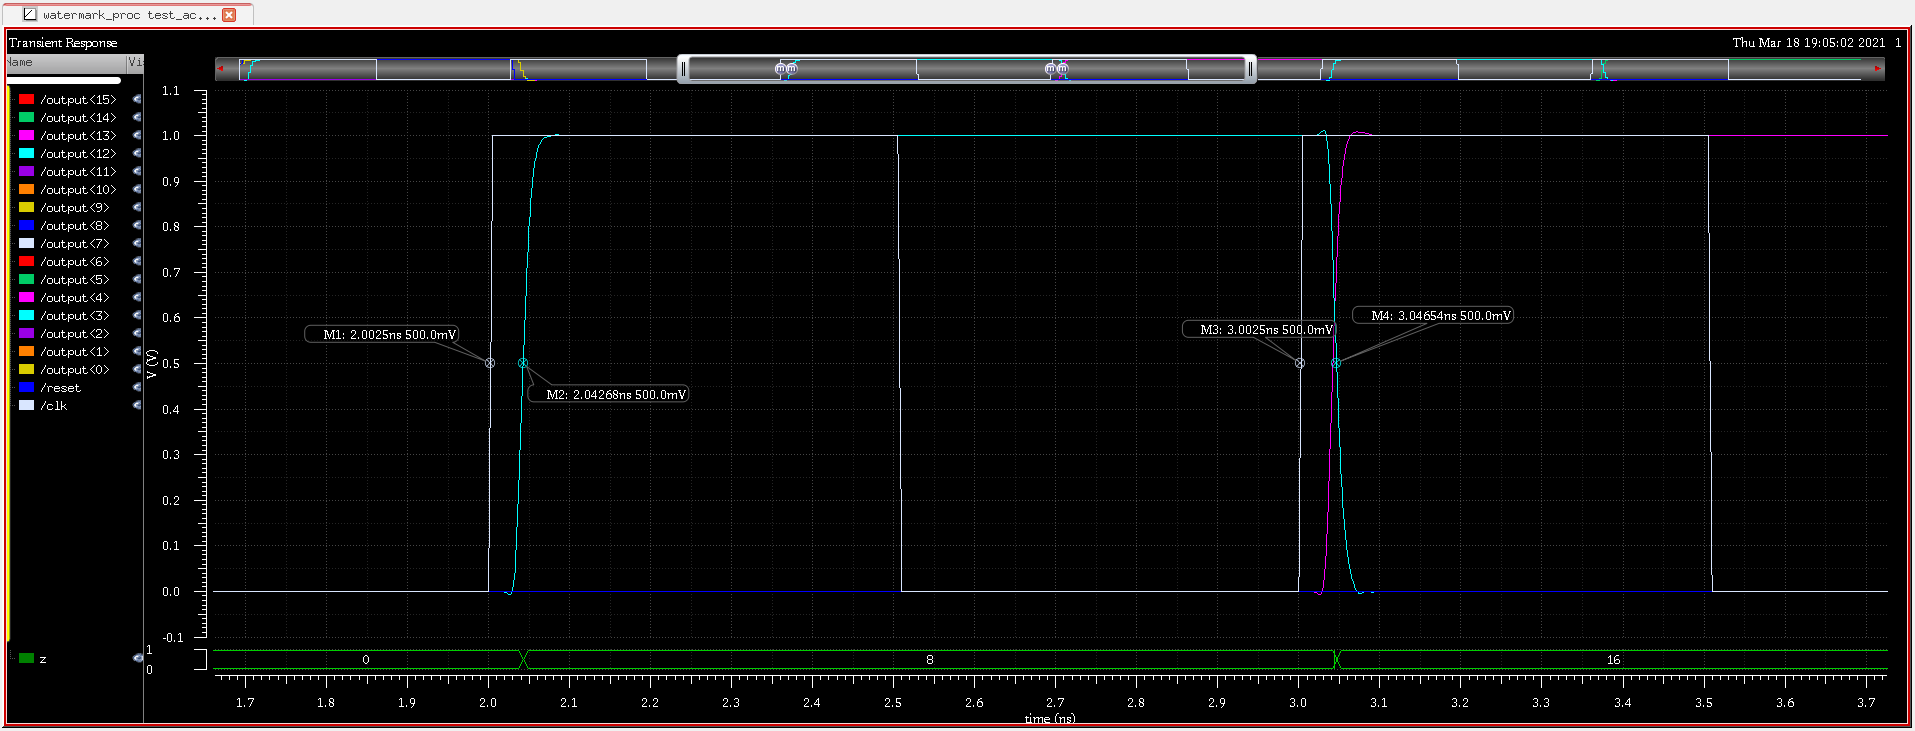
\includegraphics[width=0.85\linewidth]{report_pics/accum16b_sim.png}
		\caption{Timing of the accumulator}
		\label{fig31}
	\end{figure}
	
	\subsubsection{8-bit Comparator}
	
	The figure below (Figure \ref{fig32}) shows our functionality and timing result for the 8-bit Comparator. The unit performs as expected with the (greater or equal)'s delay of: $t_{avg\_prop} = 252.305ps$ and $t_{worst\_prop} = 293.09ps$; and the (less or equal)'s delay of: $t_{avg\_prop} = 177.04ps$ and $t_{worst\_prop} = 228.85ps$.
	
	\begin{figure}[htb!]
		\centering
		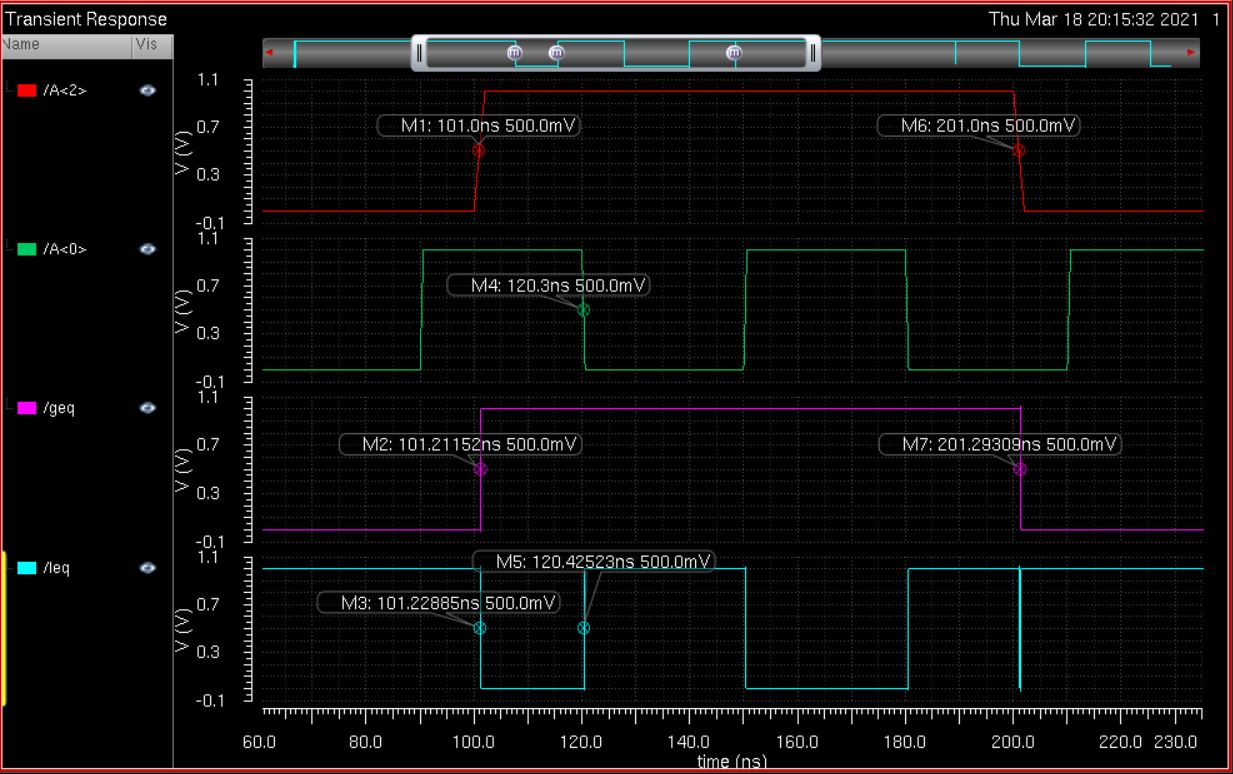
\includegraphics[width=0.85\linewidth]{report_pics/comp8b_sim.jpg}
		\caption{Simulation results of the 8-bit Comparator}
		\label{fig32}
	\end{figure}
	
	
	\subsubsection{Exponential unit}
	
	The figure below (Figure \ref{fig33}) shows our functionality and timing result for the 8-bit Exponential unit. The unit performs as expected with $t_{avg\_prop} = 674.92ps$ and $t_{worst\_prop} = 693.44ps$ 
	
	Simulating $e^{-x^2}$, with x = 0.40625 (0b00011010) returns 0b00110110 = 0.84375. The theoretical result produced by implementing Taylor series is 0.84858, so the error percentage is 0.57\%.
	
	\begin{figure}[htb!]
		\centering
		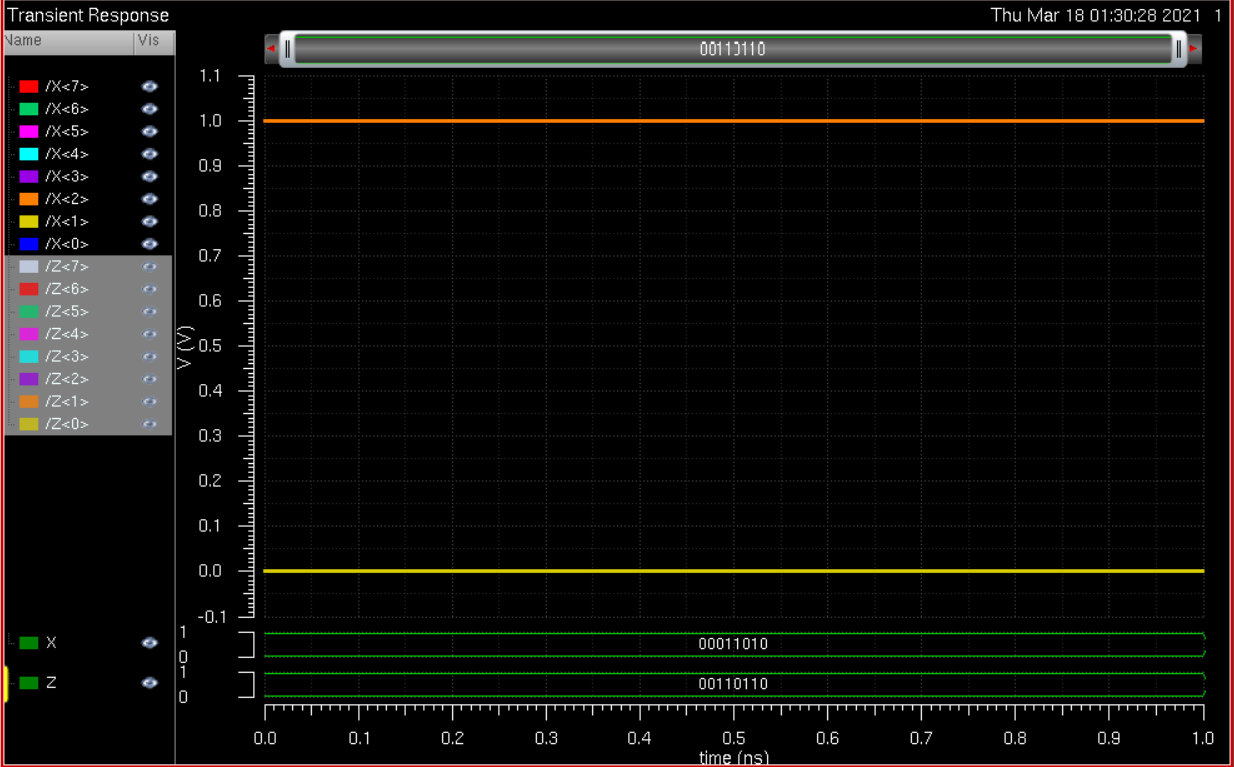
\includegraphics[width=0.85\linewidth]{report_pics/exp8b_sim.png}
		\caption{Simulation results of the 8-bit Exponential unit}
		\label{fig33}
	\end{figure}
	
	\subsubsection{Array multiplier}
	
	The figure below (Figure \ref{fig34}) shows our functionality and timing result for the 8-to-8 Array multiplier. The unit performs as expected with $t_{avg\_prop} = 184.75ps$ and $t_{worst\_prop} = 186.5ps$ 
	
	\begin{figure}[htb!]
		\centering
		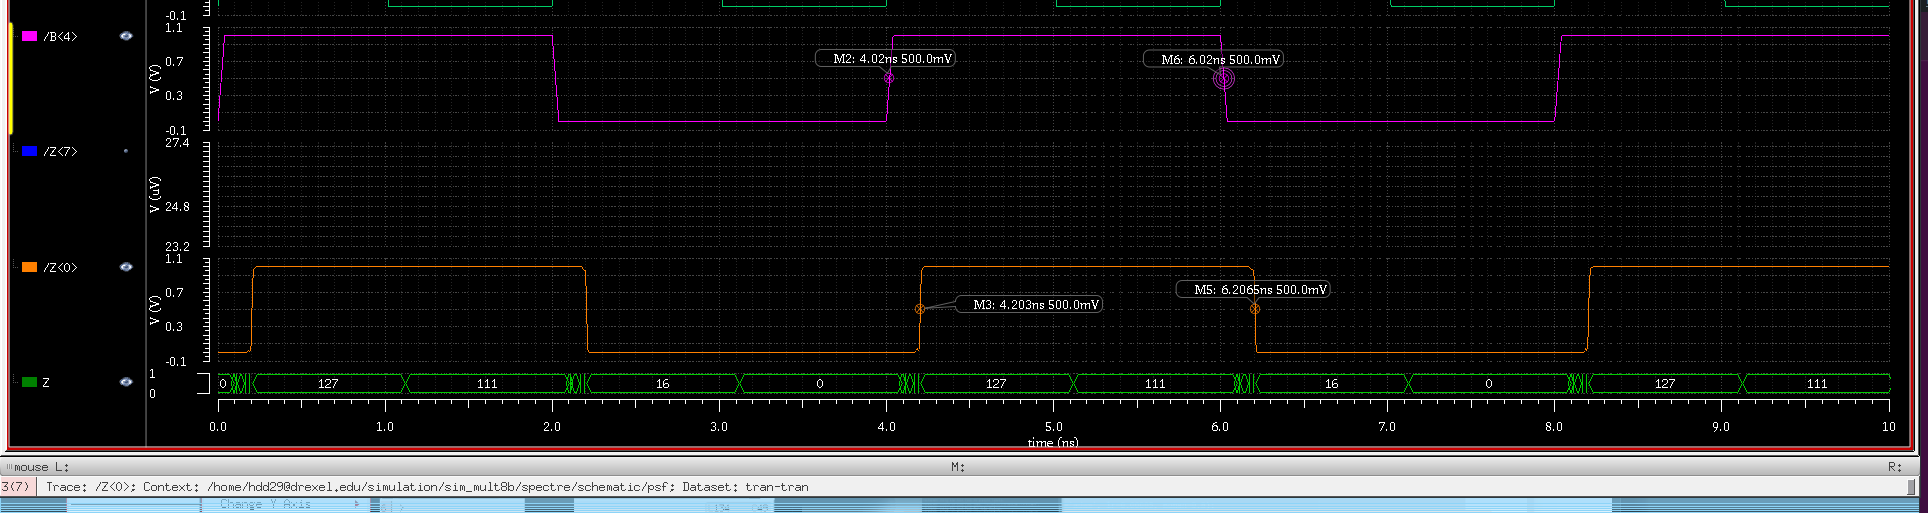
\includegraphics[width=0.85\linewidth]{report_pics/8to8_mult_sim.png}
		\caption{Simulation results of the 8-to-8 bit array multiplier}
		\label{fig34}
	\end{figure}
	
	\subsubsection{8-bit array divider}
	
	The figure below (Figure \ref{fig35}) shows our functionality and timing result for the 8-to-8 Array divider. The unit performs as expected with the quotient's delay of: $t_{avg\_prop} = 154.03ps$ and $t_{worst\_prop} = 220.1ps$; and the remainder's delay of: $t_{avg\_prop} = 158.22ps$ and $t_{worst\_prop} = 224.56ps$.
	
	\begin{figure}[htb!]
		\centering
		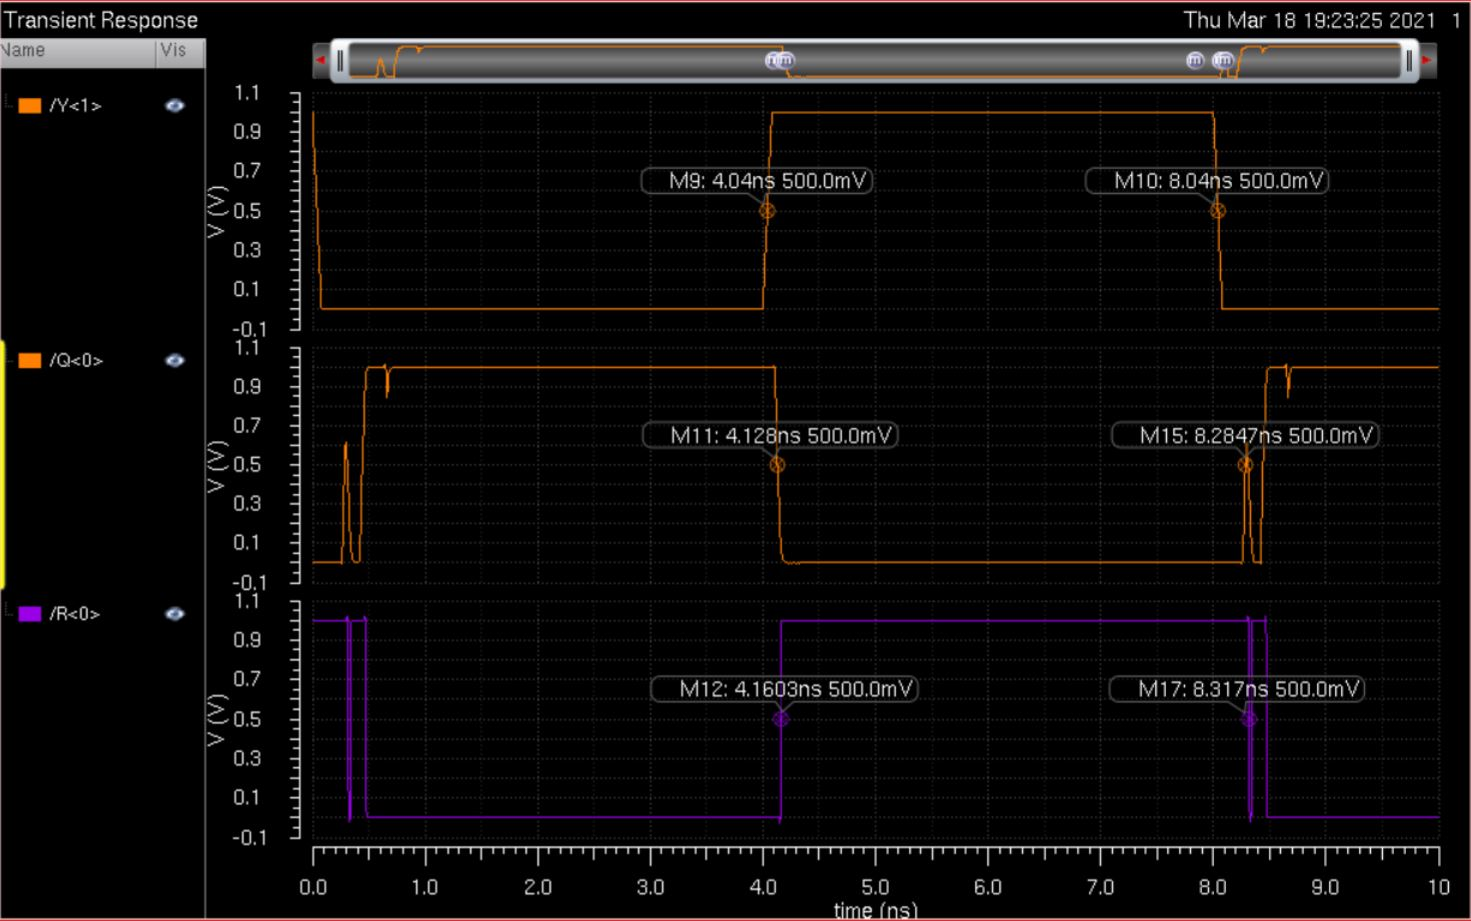
\includegraphics[width=0.85\linewidth]{report_pics/div8b_sim.JPG}
		\caption{Simulation results of the 8-to-8 bit array divider}
		\label{fig35}
	\end{figure}
	
	\newpage
	
	\subsection{Memory Blocks}
	\label{subsec:mem}
	
	\subsubsection{Memory Row}
	
	The figure below (Figure \ref{fig36}) shows our functionality and timing result for the 8-bit memory row. The unit performs as expected with the write delay of: $t_{avg\_prop} = 41.5ps$; and the read delay of: $t_{avg\_prop} = 38.3ps$.
	
	\begin{figure}[htb!]
		\centering
		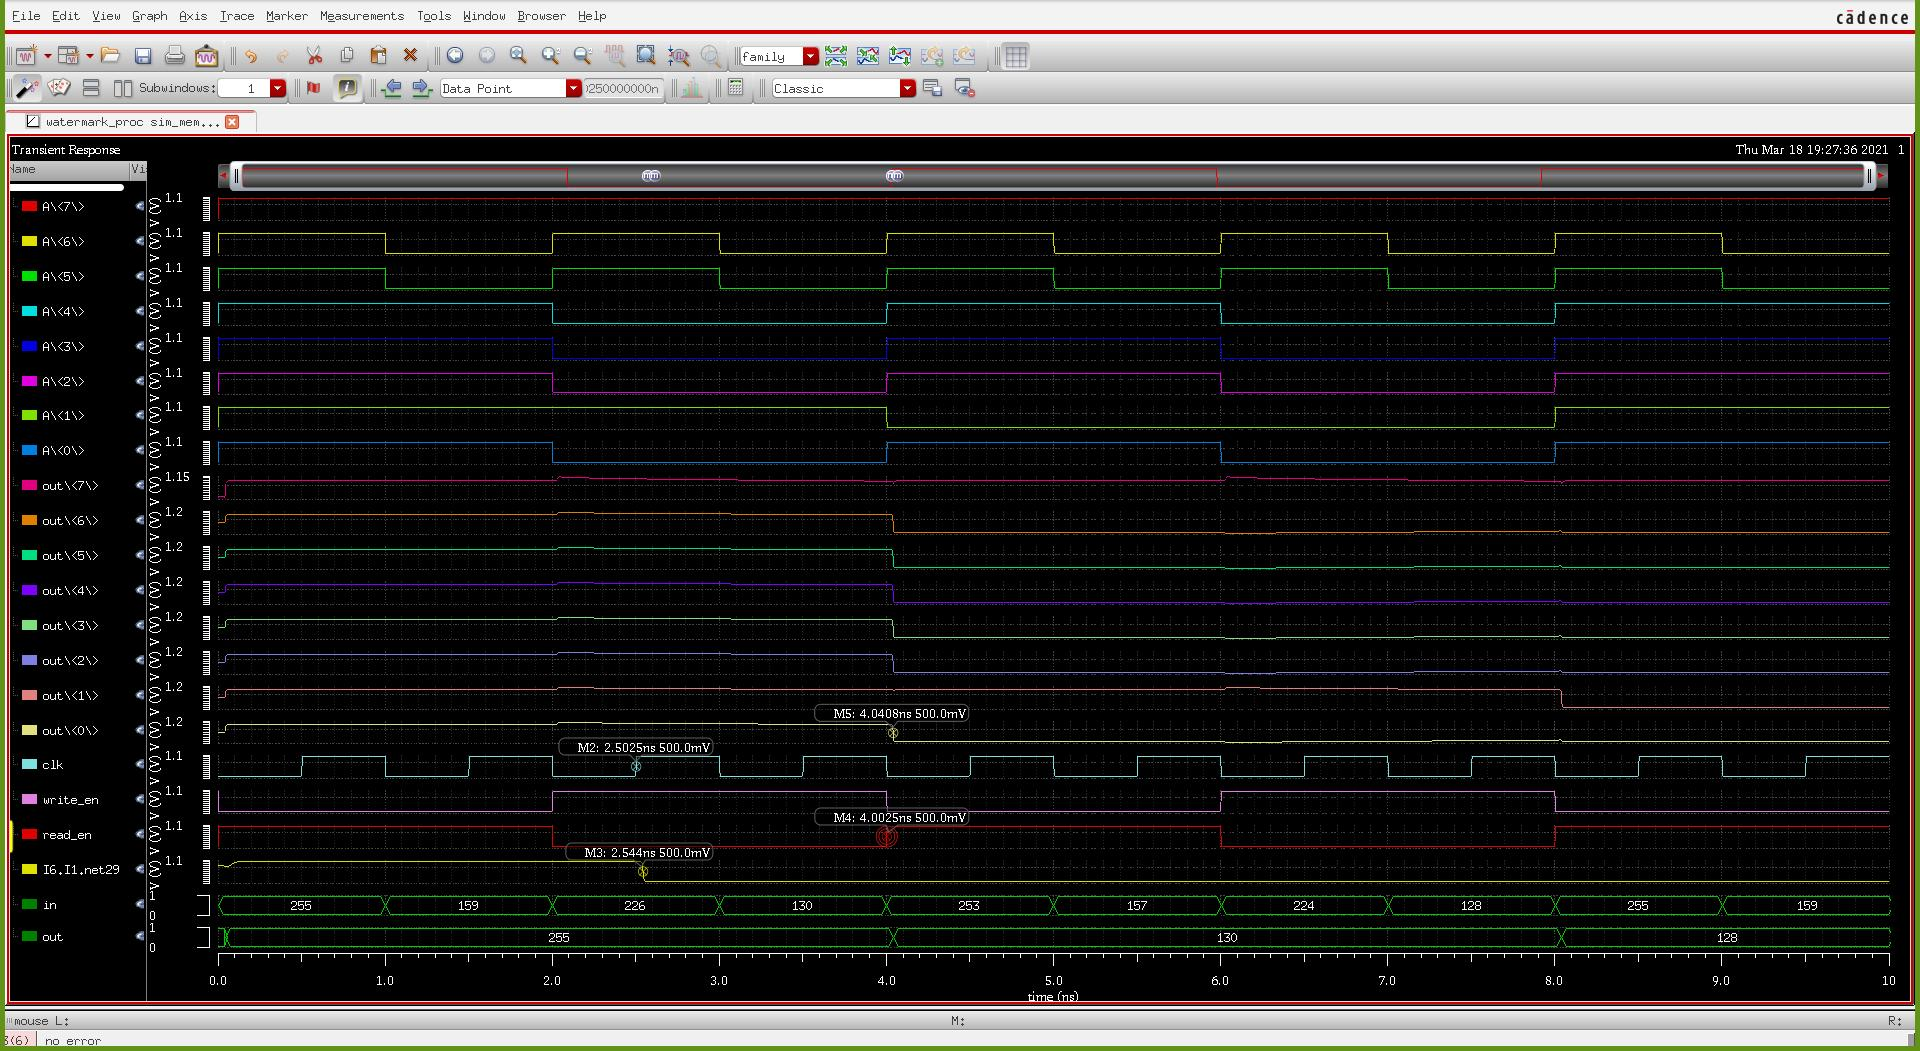
\includegraphics[width=0.85\linewidth]{report_pics/mem_row_sim.jpg}
		\caption{Simulation results of the memory row}
		\label{fig36}
	\end{figure}
	
	\subsection{Edge Detection Unit}
	\label{subsec:edge_detect}
	
	The figure below (Figure \ref{fig37}) shows our functionality and timing result for the edge detection unit. The unit performs as expected with $t_{avg\_prop} = 231.24ps$ and $t_{worst\_prop} = 240.48ps$ 
	
	\begin{figure}[htb!]
		\centering
		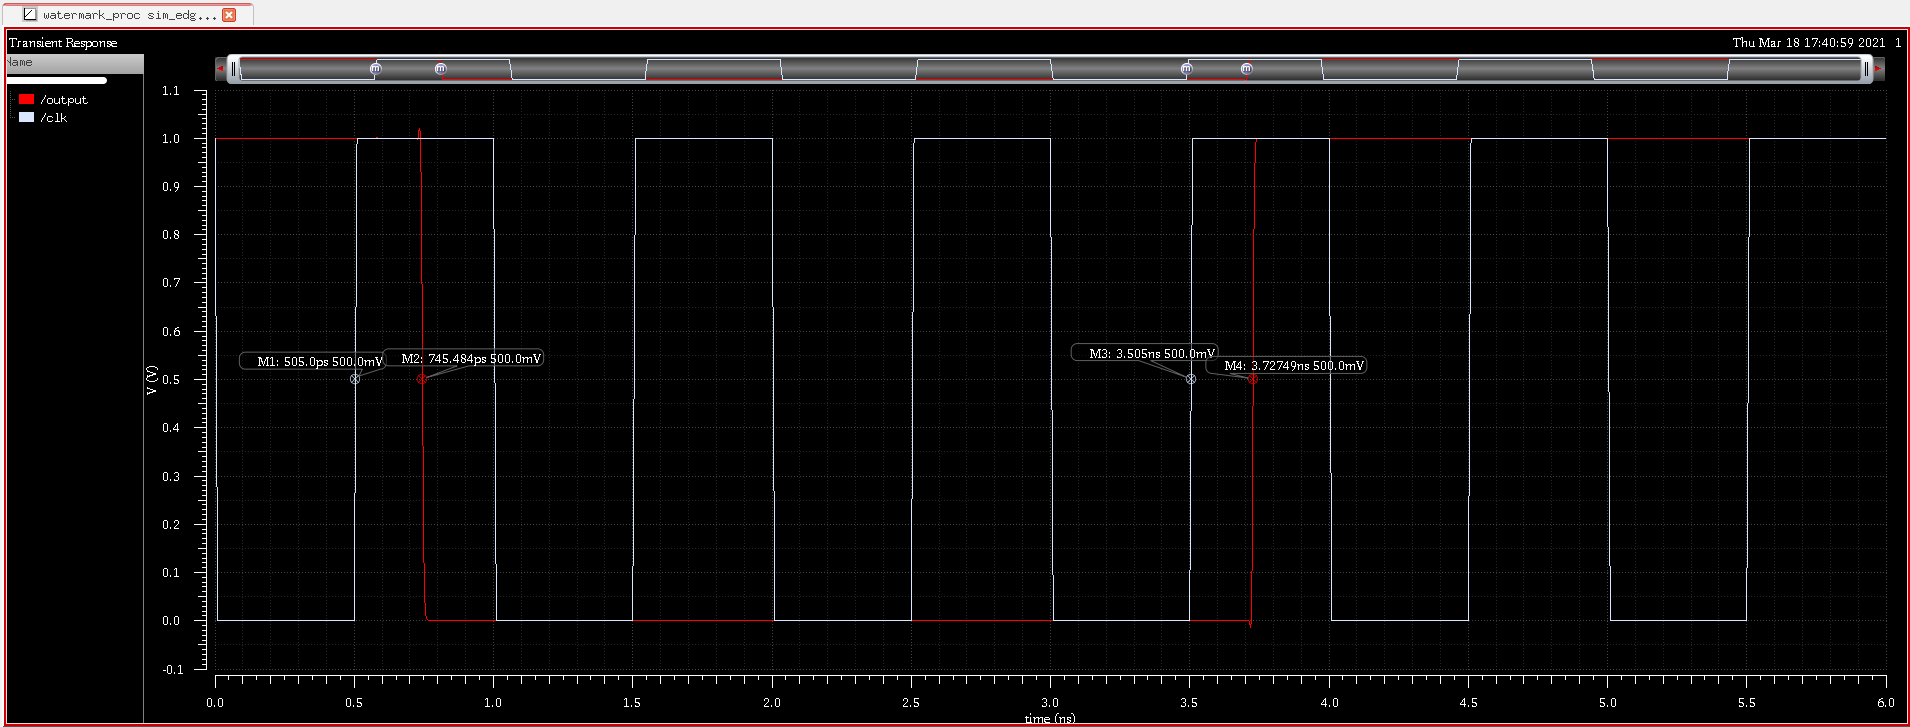
\includegraphics[width=0.85\linewidth]{report_pics/edge_detect_sim.png}
		\caption{Simulation results of the edge detection unit}
		\label{fig37}
	\end{figure}
	
	\subsection{$\alpha_k$ and $\beta_k$ Calculation Unit}
	\label{subsec:akbk}
	
	We unfortunately did not have the time resource to complete the testing using Cadence Virtuoso ADE L Schematic Simulator for the $\alpha_k$ and $\beta_k$ Calculation Unit. This is due to the fact that this unit alone comprises of over 6,000 gates, which is too big for the software to finish simulation. We waited for a full 24h but the software stuck. Hence, we aborted the running process. 
	
	However, in order to show that our design works, we have recreated the design on Cadence using Vivado 2019.2 to make sure we meet functionality requirements. Our test bench and code will be available on our project's github: https://github.com/hieumai23/watermarking-processor.
	
	\begin{figure}[htb!]
		\centering
		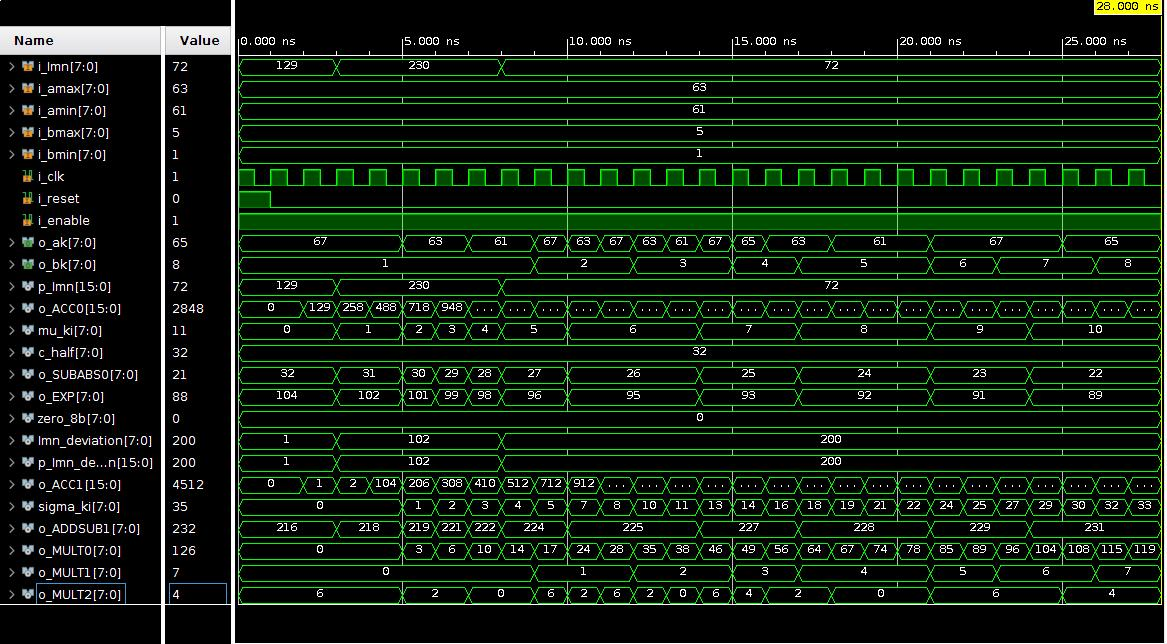
\includegraphics[width=0.85\linewidth]{report_pics/alpha_beta_vivado.jpg}
		\caption{Simulation results of $\alpha_k$ and $\beta_k$ Calculation Unit on Vivado}
		\label{fig38}
	\end{figure}
	\newpage
	In order to calculate the propagation delay for this unit, we extracted the critical path by tracing our design and choose the one with the highest delay. Since this path goes through 1 16-bit accumulator, 1 absolute substractor, 1 exponential unit, 1 divider, 1 multiplier and 1 adder-subtractor, the $t_{avg\_prop} = 1320.91ps$ and $t_{worst\_prop} = 1451.56ps$
	
	We then compared this number to the propagation delay of performing algorithm 1 (in section below), which is 895.7ps (32\% less than 1320.91ps), and found that the 2 numbers we came up with above is reasonable due to the fact that algorithm 1's critical path has about 30\% less gates than this unit.
	
	\subsection{Overall Datapath}
	\label{subsec:datapath}
	
	Similar to the $\alpha_k$ and $\beta_k$ Calculation Unit, we ran into problems simulating the entire datapath to ensure its functionality. Nonetheless, we can show that algorithm 1 (in equation \ref{eq3}) works correctly on Cadence. Algorithm 2, however, we will only show simulation results from Vivado 2019.2.
	
	\subsubsection{Algorithm 1 datapath}
	\label{subsubsec:algorithm1}
	To partially check the functionality of the datapath schematic without having to conduct transient simulation on over 6,000 gates, we created a separate datapath for only algorithm 1. The transient simulation conducted on the algorithm-1-only datapath is shown below with correct behaviour observed and timing measurements taken.  
	
	\begin{figure}[htb!]
		\centering
		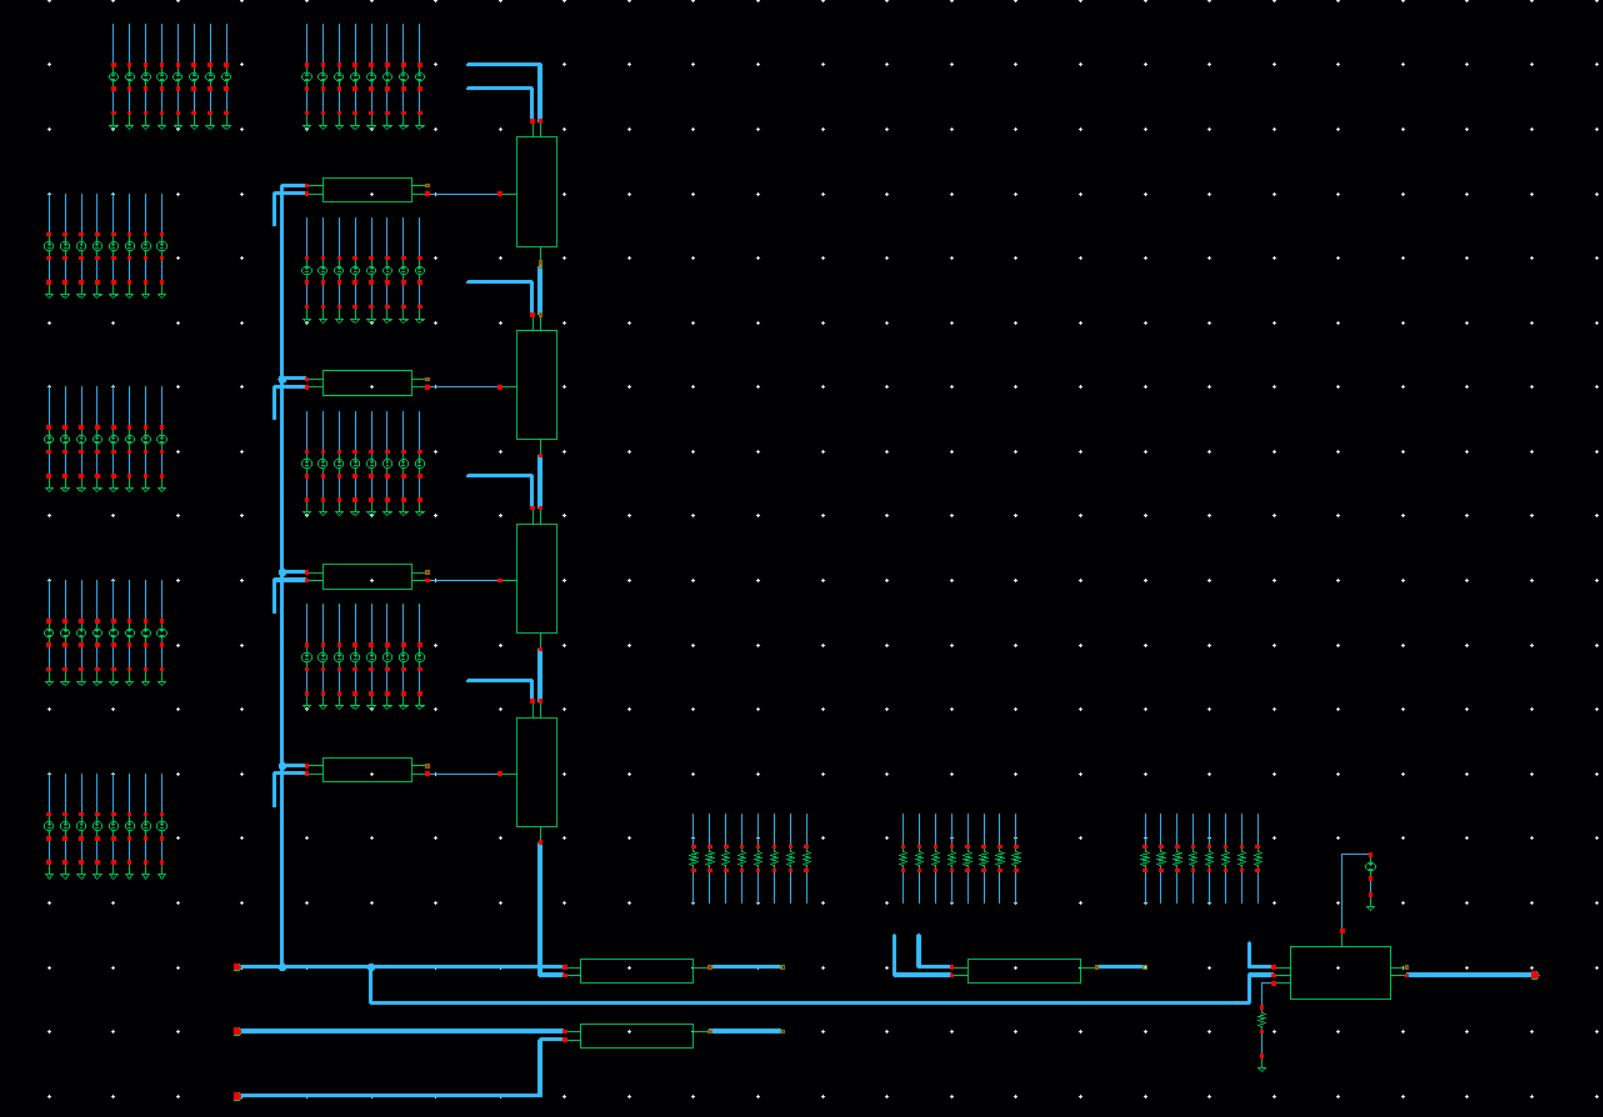
\includegraphics[width=0.85\linewidth]{report_pics/algorithm1_schem.JPG}
		\caption{Schematic of algorithm-1-only datapath}
		\label{fig39}
	\end{figure}
	\newpage
	\begin{figure}[htb!]
		\centering
		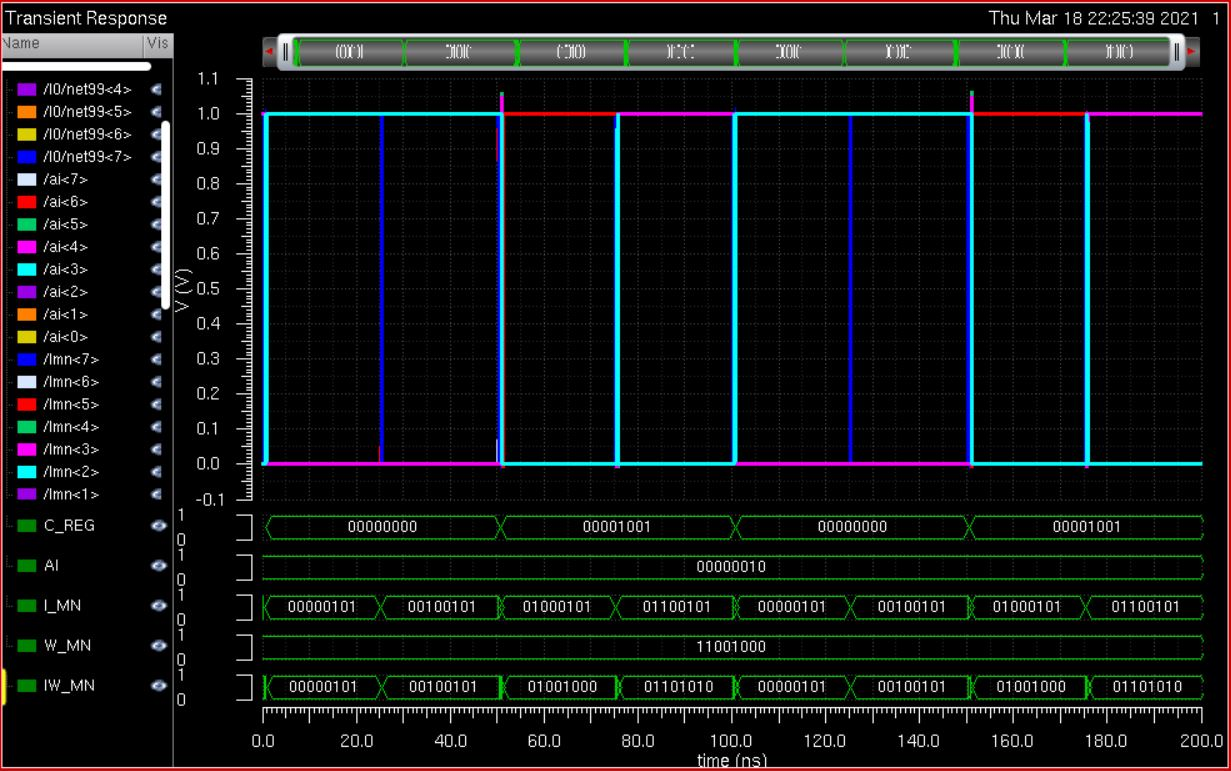
\includegraphics[width=0.85\linewidth]{report_pics/algorithm1_sim_varied_input.JPG}
		\caption{Functionality simulation of algorithm-1-only datapath}
		\label{fig40}
	\end{figure}
	
	\begin{figure}[htb!]
		\centering
		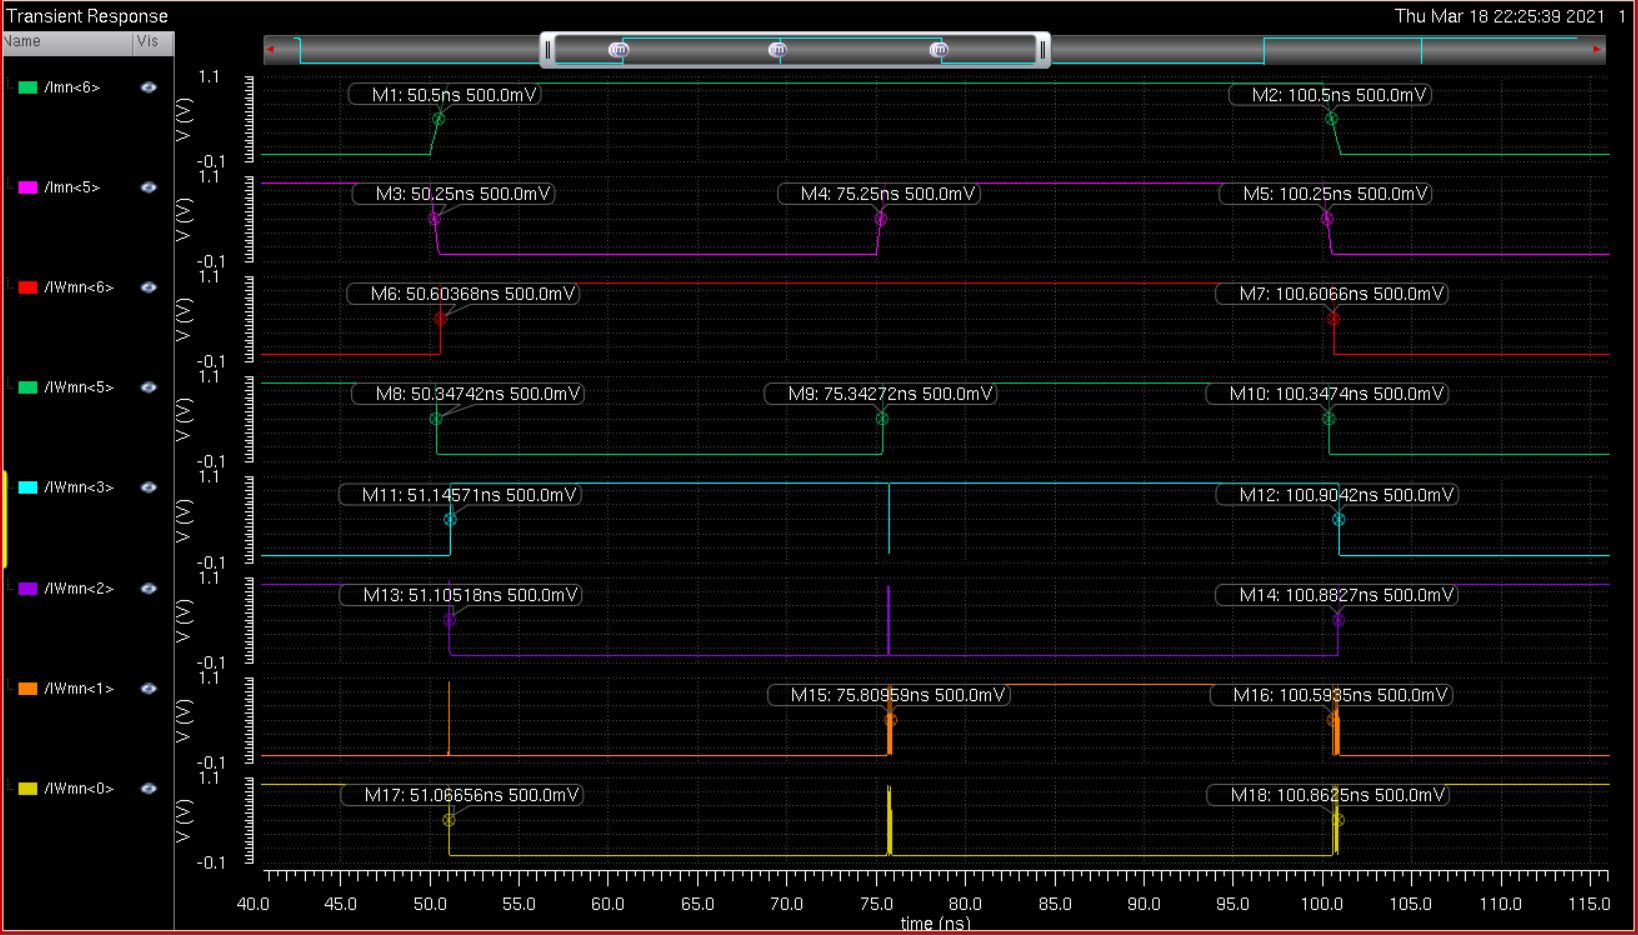
\includegraphics[width=0.85\linewidth]{report_pics/algorithm1_sim_delay.JPG}
		\caption{Timing simulation of algorithm-1-only datapath}
		\label{fig41}
	\end{figure}
	
	
	\subsubsection{Algorithm 2 datapath}
	\label{subsubsec:algorithm1}
	
	The figure below (Figure \ref{fig42}) shows our algorithm 2 datapath simulation on Vivado 2019.2.
	
	\begin{figure}[htb!]
		\centering
		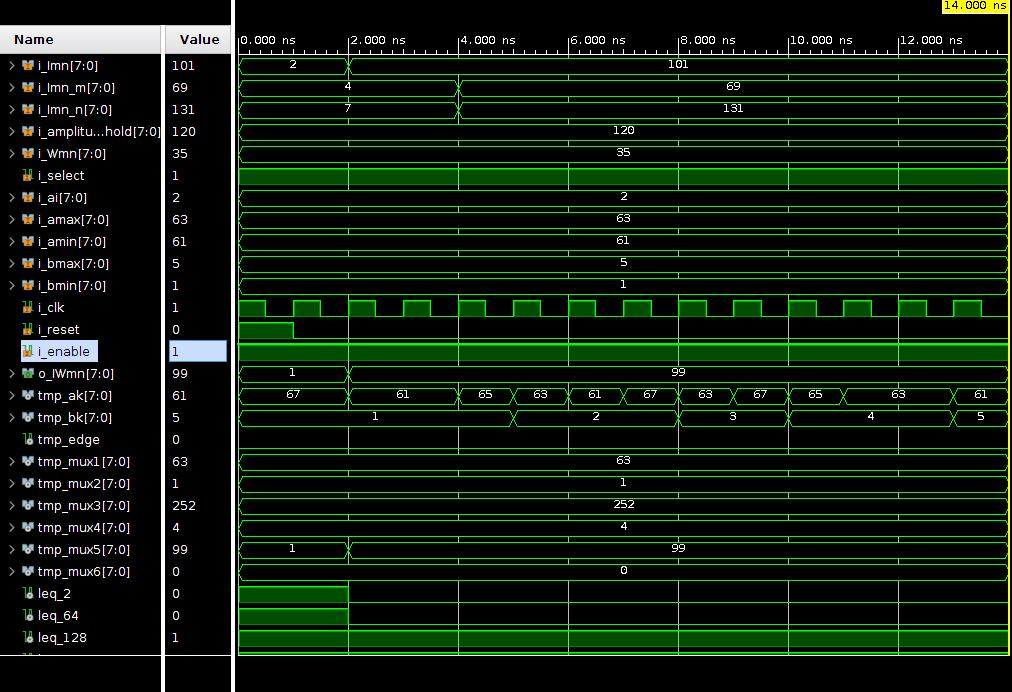
\includegraphics[width=0.85\linewidth]{report_pics/datapath_algo2_vivado.jpg}
		\caption{Simulation results of Algorithm 2 Datapath on Vivado}
		\label{fig42}
	\end{figure}
	
	\newpage
	\subsection{Controller}
	\label{subsec:controller}
	Pictures of Vivado simulations algorithm 1 and 2
	\begin{figure}[htb!]
		\centering
		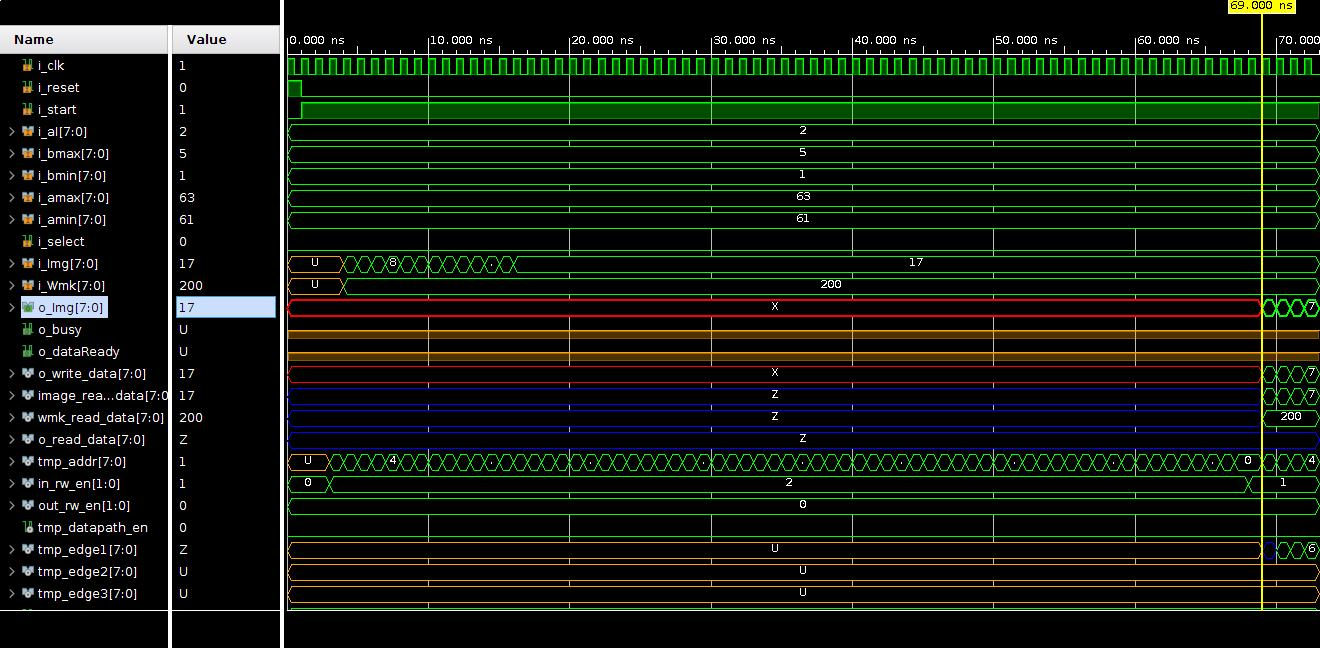
\includegraphics[width=0.85\linewidth]{report_pics/controller_algo1_vivado.jpg}
		\caption{Simulation results of Algorithm 1 Controller on Vivado}
		\label{fig43}
	\end{figure}
	
	\begin{figure}[htb!]
		\centering
		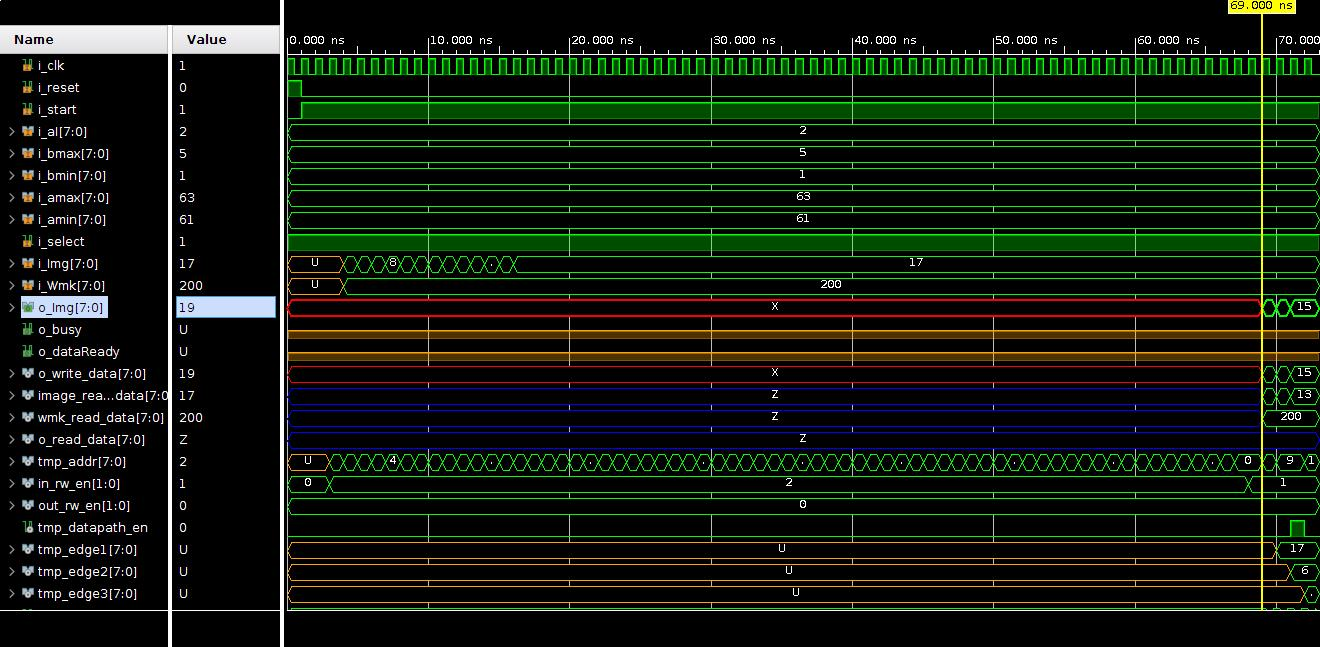
\includegraphics[width=0.85\linewidth]{report_pics/controller_algo2_vivado.jpg}
		\caption{Simulation results of Algorithm 2 Controller on Vivado}
		\label{fig44}
	\end{figure}
	
	\newpage
	\section{Testing Summary}
	\label{sec:testsumm}
	
	In this section, we will summarize our testing here with 2 tables. The first table will show our experiments in order to extract timing (delays) and power consumption. The second table will compare our design with paper \cite{1}'s design in terms of number of gates:
	
	*The power consumption for each of these units is extrapolated from the power consumption for their sub-units.
	
	**The total number of gate for our design is extracted by taking the total number of gates for the overall datapath + the number of gates for 3 memory blocks: (to store the original image, the watermark image, and the final image).
	
	***We did not have time to complete power analysis for these units.
	
	\begin{table}
		\label{table1}
		\caption{Table showing timing result}
		\centering
		\begin{tabular}{llllll}
			Net name & Pos.Delay(ps) & Neg.Delay(ps) & Avg.Delay(ps) & Worst Delay(ps) & Power($\mu W$) \\ 
			\hline
			Addsub\_8b & 105.4 & 131.94 & 118.67 & 131.94 & 55.32\\
			Add\_16b & 103.39 & 153.95 & 128.67 & 153.95 & 112.20\\
			Accum\_16b & 40.18 & 44.04 & 42.11 & 44.04 & 150.46 \\
			Multiplier 8-to-8 & 183 & 186.5 & 184.75 & 186.5 & 16.81 \\
			Divider (quotient) & 220.1 & 87.96 & 154.03 & 220.1 & 501.39* \\
			Divider (remainder) & 224.56 & 91.88 & 158.22 & 224.56 & 501.39* \\
			Exponential & 656.4 & 693.44 & 674.92 & 693.44 & 163.60* \\
			Absolute\_diff & 117.31 & 175.54 & 146.425 & 175.54 & 58.27 \\
			Compare\_8b (geq signal) & 211.52 & 293.09 & 252.305 & 293.09 & 3.85 \\
			Compare\_8b (leq signal) & 125.23 & 228.85 & 177.04 & 228.85 & 3.51 \\
			Compare\_8b & 211.52 & 293.09 & 252.305 & 293.09 & 7.35 \\
			Edge\_detect & 240.48 & 222 & 231.24 & 240.48 & 323.77* \\
			Mem\_row & 41.5 & 38.3 & 39.9 & 41.5 & N/A*** \\
			Alpha beta & 1322.39 & 1319.42 & 1320.905 & 1322.39 & 1291.51* \\
			Datapath algo 1 & 895.70 & 855.18 & 875.44 & 895.70 & N/A*** \\
			Datapath overall & 1976.79 & 2010.86 & 1993.825 & 2010.86 & 1750.64* \\ 
			\hline
		\end{tabular}
	\end{table}
	
	
	
	\begin{table}
		\label{table2}
		\caption{Table showing gate count result extracted from Cadence Virtuoso Layout Generation tool}
		\centering
		\begin{tabular}{lll}
			Block name & Our number of gates & Paper \cite{1} number of gates \\ 
			\hline
			Memory block & 2950 & N/A \\
			Edge detection & 1136 & 3599 \\
			Exponential unit & 1716 & 2370 \\
			Alpha beta unit & 6924 & 16279  \\
			Datapath algorithm 1 & 4916 & N/A\\
			Overall datapath & 10402 & N/A \\
			\hline
			Total & 19252** & 28469 \\                 
			\hline
		\end{tabular}
	\end{table}
	
	\newpage
	\begin{figure}[htb!]
		\centering
		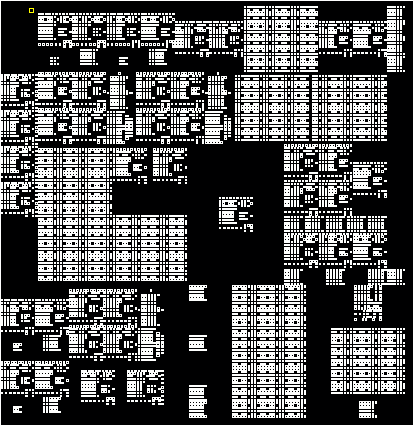
\includegraphics[width=0.85\linewidth]{report_pics/datapath_layout.png}
		\caption{Overall datapath layout on Cadence Virtuoso Layout Generation tool (area of 0.407mm x 0.423mm and 10402 gates)}
		\label{fig45}
	\end{figure}
	
	\begin{figure}[htb!]
		\centering
		\includegraphics[width=0.85\linewidth]{report_pics/mem_block_layout.png}
		\caption{Memory block layout on Cadence Virtuoso Layout Generation tool (area of 0.217mm x 0.294mm and 2950 gates)}
		\label{fig46}
	\end{figure}
	
	\newpage
	\section{Optimization}
	\label{sec:optimization}
	\subsection{Hardwired constants}
	\label{subsec:hardwire_constants}
	In the reference paper, all the constants used in the datapath are stored in a small register file and only fetched when needed. In contrast, our design hard wired all the constants for ease of controller design, and reduction in overall delay as there is no delay in transferring the data from the register file to the destination. This might be a trade off in power and customizability as the constants are always draining from VDD and VSS, and they cannot be adjusted if the algorithm changes these parameters. Further work would involve power and delay analysis on cases of using register file in comparison with the hard wired constants.
	
	\subsection{Customize fixed-point format}
	\label{subsec:custom_fixed_point}
	Based on a thorough study of the architecture of complex units like $\alpha_k$ and $\beta_k$ calculation and overall datapath, two different formats of fixed-point real numbers are implemented throughout the design process. For $\alpha_k$ and $\beta_k$ calculation unit, the variables of this computation process range from very small decimal numbers to over 1.5, so the format used in this unit is 2Q6, which maintains a good accuracy for small number and is capable of holding numbers within 1 and 2 with high accuracy. Outside of this unit, the variables are either integer within 0 and 255, representing the value of a pixel, or decimal numbers that fall within 0 and 1. Therefore, in the overall datapath, the integers are kept in unsigned decimal format, and the decimal numbers are represented in 0Q8 format, which allows a better accuracy throughout the computation without any risk of losing data. 
	Thanks to this customization, the data is processed at high accuracy and high speed. 
	
	\subsection{Remove multipliers when multiplying with $2^{-x}$}
	\label{subsec:bit_mapping}
	
	As highlighted in the design section, some multipliers whose multiplicand is a constant of the form $2^{-x}$, where x is a positive integer, is removed. The output of the block prior to the multiplier is “mapped” in a special way to the input of the block after the multiplier. 
	
	Using this optimization, we have successfully reduced the power consumption by $33.624 \mu$W by removing 2 multipliers in the alpha beta calculation unit, and an additional $16.81 \mu W$ by removing 1 multiplier in the edge detection unit to get a total power reduction of $50.44 \mu W$ . In addition to the reduction in power, there is also a reduction in the number of gates needed for the blocks. Since there is 512 gates in each multiplier, overall we have reduced the number of total gates used for the datapath by 1536 gates just by the bit-mapping method.
	
	\subsection{Use 1V voltage source}
	\label{subsec:use1V}
	
	As the application calls for only accuracy but not time-critical, and a smaller technology node is used in our design,we chose a lower voltage source of 1V instead of the 3.3V used in the reference paper [1]. This lower voltage source would optimize for the power consumption of the watermarking chip by reducing it by around 3 times, with a trade off in threshold voltage, increasing the switching delay of transistors. 
	
	\newpage 
	\section{Conclusion}
	\label{sec:conclusion}
	The design of the visible watermarking processor integrating the 2 algorithms by Mohanty [3] and Meng and Chang [2] is successfully implemented in our design following Mohanty reference VLSI design of the same chip [1] with a change in technology node and various optimization made. The design was verified in Cadence Virtuoso Schematic and Layout Suit and partly in Vivado Digital Design Suite (for functionality verification purposes only). A total datapath area of 0.407mm x 0.423mm and total datapath power consumption of 1.75348 mW  was estimated using Cadence's layout generation tool and multiplication of current and voltage in Cadence Virtuoso Schematic ADE L transient simulation.
	
	Compared to the design proposed in [1], our design has a lower number of gates. However, this might be incorrect, because we have not fully generated the layout with ICC tools in order to perform post-placement processes such as: global/local/detail routing, clock tree synthesis (cts), post-cts, and layout extraction.
	
	Our reported datapath power consumption is also significantly lower than in [1], which is mostly attributed to the technology node that was used (45nm vs 350nm). However, our method of estimating power consumption does not give a good estimation, as we only multiply the voltage and current observed at the output. This could be inaccurate because it does not account for the power consumption on the path that the input signals propagate through; we also only tested each unit with a limited set of input signals, and our number only represents the power consumption for those specific cases.
	
	Some of the challenges that we faced during this project include long simulation time, lagginess due to having to access the server over VPN, and difficulty in functionality testing for high-frequency systems. The technical knowledge required to complete this project is also a big challenge, especially for the integration of datapath with the controller. We have overcome this challenge by performing both simulations on Cadence Virtuoso and Vivado Design Suite, but unable to finish in time due to the amount of time it takes to run ADE simulations.
	
	For further improvement, we could perform more accurate power/timing/area estimation using ICC tools. Due to limited time resource and limited experience in the field, we were only able to provide "ball-park" numbers. In addition, if we had more time, we would look into writing code in Verilog in order to use existing ICC tools on Drexel's server, which would allow us to perform actual chip synthesis and extract a layout good enough for manufacturing. If we could load our design on to these automated tools, then we can optimize for power, delay, and area by applying routing algorithms (Particle Swarm Optimization, Ant Colony Optimization), clock-tree optimization algorithms, and post-cts algorithms (inserting buffers, 3D layer assignment) so that our design can have better performance. 
	
	\newpage
	\begin{thebibliography}{9}
		\bibitem{1}
		Mohanty, S.P., et al. “A VLSI Architecture for Visible Watermarking in a Secure Still Digital Camera (S/Sup 2/DC) Design (Corrected)*.” IEEE Transactions on Very Large Scale Integration (VLSI) Systems, vol. 13, no. 8, 2005, pp. 1002–1012., doi:10.1109/tvlsi.2005.857991.
		\bibitem{2}
		Meng, Jianhao, and Chang, Shih-Fu. “Embedding Visible Video Watermarks in the Compressed Domain.” Proceedings 1998 International Conference on Image Processing. ICIP98 (Cat. No.98CB36269), 1998, doi:10.1109/icip.1998.723534.
		\bibitem{3}
		Mohanty, Saraju P., et al. “A Dual Watermarking Technique for Images.” Proceedings of the Seventh ACM International Conference on Multimedia (Part 2)  - MULTIMEDIA '99, 1999, doi:10.1145/319878.319891.
		\bibitem{4}
		“Tri-State-Buffers.” CS355 Sylabus, www.mathcs.emory.edu/~cheung/Courses/355/Syllabus/3-memory/tri-state.html. 
		\bibitem{5}
		Yu-Ting Pai, and Yu-Kumg Chen. “The Fastest Carry Lookahead Adder.” Second IEEE International Workshop on Electronic Design, Test and Applications, doi:10.1109/delta.2004.10071. 
		\bibitem{6}
		Narendra, K, et al. “FPGA Implementation of Fixed Point Integer Divider Using Iterative Array Structure.” International Journal of Engineering and Technical Research (IJETR), vol. 3, no. 4, Apr. 2015, pp. 170–179. 
		
	\end{thebibliography}
	
\end{document}